% !TeX spellcheck = en_GB
%%% The main file. It contains definitions of basic parameters and includes all other parts.

%% Settings for single-side (simplex) printing
% Margins: left 40mm, right 25mm, top and bottom 25mm
% (but beware, LaTeX adds 1in implicitly)
\documentclass[final,12pt,a4paper]{report}
\setlength\textwidth{145mm}
\setlength\textheight{247mm}
\setlength\oddsidemargin{15mm}
\setlength\evensidemargin{15mm}
\setlength\topmargin{0mm}
\setlength\headsep{0mm}
\setlength\headheight{0mm}
% \openright makes the following text appear on a right-hand page
\let\openright=\clearpage

%% Settings for two-sided (duplex) printing
% \documentclass[12pt,a4paper,twoside,openright]{report}
% \setlength\textwidth{145mm}
% \setlength\textheight{247mm}
% \setlength\oddsidemargin{14.2mm}
% \setlength\evensidemargin{0mm}
% \setlength\topmargin{0mm}
% \setlength\headsep{0mm}
% \setlength\headheight{0mm}
% \let\openright=\cleardoublepage

%% Generate PDF/A-2u
\usepackage[a-2u]{pdfx}

%% Character encoding: usually latin2, cp1250 or utf8:
\usepackage[utf8]{inputenc}

%% Prefer Latin Modern fonts
\usepackage{lmodern}

%% Further useful packages (included in most LaTeX distributions)
\usepackage{amsmath}        % extensions for typesetting of math
\usepackage{amsfonts}       % math fonts
\usepackage{amsthm}         % theorems, definitions, etc.
\usepackage{bbding}         % various symbols (squares, asterisks, scissors, ...)
\usepackage{bm}             % boldface symbols (\bm)
\usepackage{graphicx}       % embedding of pictures
\usepackage{fancyvrb}       % improved verbatim environment
\usepackage{natbib}         % citation style AUTHOR (YEAR), or AUTHOR [NUMBER]
\usepackage[nottoc]{tocbibind} % makes sure that bibliography and the lists
			    % of figures/tables are included in the table
			    % of contents
\usepackage{dcolumn}        % improved alignment of table columns
\usepackage{booktabs}       % improved horizontal lines in tables
\usepackage{paralist}       % improved enumerate and itemize
\usepackage{xcolor}         % typesetting in color
\usepackage{tikz}
\usetikzlibrary{arrows.meta, positioning, fit, shapes.geometric}
\usepackage{cleveref}
\usepackage{float}
\usepackage{listings}
\usepackage{subcaption}
\usepackage[edges]{forest}

\forestset{
	filesystem/.style={
		for tree={
			grow'=0,
			parent anchor=east,
			child anchor=west,
			anchor=west,
			edge={-},
			font=\ttfamily\small,
			l sep=10pt,
			s sep=3pt,
			inner sep=1pt
		}
	}
}
\usepackage{dirtree}
\usetikzlibrary{positioning}
\usetikzlibrary{arrows}
\usepackage[ruled]{algorithm2e}
%%% Basic information on the thesis

% Thesis title in English (exactly as in the formal assignment)
\def\ThesisTitle{Fitness and novelty in evolutionary reinforcement learning}

\def\ThesisTitleCz{Fitness a novelty v evolučním zpětnovazebném učení}
% Author of the thesis
\def\ThesisAuthor{Bc. František Dostál}

% Year when the thesis is submitted
\def\YearSubmitted{2026}

% Name of the department or institute, where the work was officially assigned
% (according to the Organizational Structure of MFF UK in English,
% or a full name of a department outside MFF)
\def\Department{Department of Theoretical Computer Science and Mathematical Logic}

\def\DepartmentCz{Katedra teoretické informatiky a matematické logiky}

% Is it a department (katedra), or an institute (ústav)?
\def\DeptType{Department}
\def\DeptTypeCz{Katedra}
% Thesis supervisor: name, surname and titles
\def\Supervisor{Mgr. Roman Neruda, CSc.}

% Supervisor's department (again according to Organizational structure of MFF)
\def\SupervisorsDepartment{Department of Theoretical Computer Science and Mathematical Logic}

\def\SupervisorsDepartmentCz{Katedra teoretické informatiky a matematické logiky}
% Study programme and specialization
\def\StudyProgramme{Informatics}
\def\StudyBranch{Artificial Intelligence}

% An optional dedication: you can thank whomever you wish (your supervisor,
% consultant, a person who lent the software, etc.)
\def\Dedication{%
I would like to thank my supervisor Mgr. Roman Neruda, CSc. for patience and guidance. I would also like to thank  my friend Martin Mečiar for moral support when it was most needed.
}

% Abstract (recommended length around 80-200 words; this is not a copy of your thesis assignment!)
\def\Abstract{%
This thesis investigates the use of novelty in evolutionary algorithms on reinforcement learning tasks. We compare novelty-based with fitness-based selection, their archival variants and dynamic combinations of novelty and fitness on Gymnasium environments CartPole and Lunar Lander. For each environment we define an interpretable behavioural characteristic and examine how the choice of objective handling method affects the resulting fitness and population diversity.
The results show the fitness-based methods achieve best performance under the experiment conditions. The novelty increases population diversity but its benefit depends on specific task dynamics. 
The thesis also discusses sensitivity of novelty search to the choice of behavioural space and interactions between the environment and the evolutionary algorithm. 
}

\def\AbstractCz{%
	Tato práce zkoumá využití novelty v evolučních algoritmech při řešení úloh zpětnovazebního učení. Porovnává selekci založenou na novelty se selekcí založenou na fitness, jejich variantami využívajícími archivy a dynamickými kombinacemi novelty a fitness. Porovnání probíhá na prostředích CartPole a Lunar Lander z knihovny Gymnasium. Pro každé prostředí definujeme interpretovatelnou behaviorální charakteristiku a analyzujeme vliv jednotlivých metod práce s objektivní funkcí na dosaženou fitness a diverzitu populace.
	Výsledky ukazují, že metody založené na fitness představují nejsilnější výchozí přístup z hlediska dosaženého výkonu. Využití novelty zvyšuje diverzitu populace, avšak její přínos závisí na dynamice konkrétní úlohy.
	Práce dále diskutuje citlivost výsledků algoritmů založených na novelty na volbu behaviorálního prostoru a vzájemné interakce mezi prostředím a evolučním algoritmem.
	
}

% 3 to 5 keywords (recommended), each enclosed in curly braces
\def\Keywords{%
{evolution};{novelty}; {fitness}; {behavioural space}
}

\def\KeywordsCz{%
	{evoluce}; {novelty}; {fitness}; {behaviorální prostor}
}

%% The hyperref package for clickable links in PDF and also for storing
%% metadata to PDF (including the table of contents).
%% Most settings are pre-set by the pdfx package.
\hypersetup{unicode}
\hypersetup{breaklinks=true}

% Definitions of macros (see description inside)
\include{macros}

% Title page and various mandatory informational pages
\begin{document}

\include{title}

%%% A page with automatically generated table of contents of the master thesis

\tableofcontents

%%% Each chapter is kept in a separate file
% !TeX spellcheck = en_GB
\chapter*{Introduction}
\addcontentsline{toc}{chapter}{Introduction}

Evolutionary algorithms (EAs) are a class of optimization and search techniques inspired by the principles of natural evolution. Over the past decades, these algorithms have been successfully applied to a wide range of complex problems in engineering, robotics, and machine learning. Their ability to explore large and poorly understood search spaces makes them particularly suitable for problems where traditional optimization methods are applied only with great difficulty.

The performance of evolutionary algorithms is typically driven by a objective function, which evaluates candidate solutions according to predefined objectives. In classical evolutionary computation, this is usually refered to as fitness-based selection. While this approach has proven effective in many domains, it also presents several limitations. In particular, fitness-driven search can suffer from premature convergence, stagnation in local optima, and deception, where the search process becomes trapped in regions that appear promising but ultimately prevent discovery of globally optimal solutions.

To address these challenges, alternative search paradigms have been proposed, among which novelty search has gained significant attention. Unlike traditional fitness-based optimization, novelty search rewards behavioral uniqueness rather than objective performance. Introduced as a method to overcome deception in evolutionary search, novelty search encourages exploration by promoting individuals whose behaviors differ from those previously encountered. This shift from objective-oriented optimization to exploration-oriented search has demonstrated promising results in domains characterized by sparse rewards, deceptive landscapes, and high-dimensional complexity.

The distinction between fitness-based and novelty-driven approaches reflects two fundamentally different philosophies of evolutionary search. Fitness-oriented methods prioritize exploitation of known promising regions in the search space, whereas novelty-based methods emphasize exploration and behavioral diversity. Both approaches offer unique advantages and disadvantages depending on the characteristics of the problem domain. Fitness-based methods generally provide faster convergence toward measurable objectives but may lack robustness in deceptive environments. Novelty search, on the other hand, can discover innovative and unexpected solutions, although it may require greater computational resources and may struggle in tasks where exploration alone is insufficient.

This thesis focuses on a comparative analysis of novelty and fitness mechanisms in evolutionary algorithms when applied to reinforcement learning tasks. The objective is to investigate how these approaches influence search dynamics´, convergence behavior, diversity maintenance, and solution quality across selected optimization problems. The study aims to identify conditions under which novelty search outperforms traditional fitness-based evolution, as well as scenarios where fitness-driven optimization remains more effective.

The research combines theoretical analysis with experimental evaluation. Several benchmark problems and simulation environments are employed to compare the behavior of both methods under controlled conditions. Metrics such as convergence speed, population diversity, robustness, and final solution quality are analyzed to provide a comprehensive understanding of the strengths and limitations of each approach. Additionally, hybrid methods that combine novelty and fitness objectives are considered to examine whether balancing exploration and exploitation can improve overall evolutionary performance.

The findings of this thesis contribute to the broader understanding of exploration and exploitation trade-offs in evolutionary computation. By examining the relationship between novelty and fitness, this work seeks to provide insights into the design of more adaptive and efficient evolutionary algorithms capable of solving increasingly complex optimization problems.

\include{theory}
% !TeX spellcheck = en_GB
\chapter{Environments}
\label{chap:environment}

\section{Reinforcement learning}
Reinforcement learning might be best introduced by description of the problem it aims to solve.
\begin{defn}[Markov’s decision problem]
We define Markov’s decision problem (MDP) by a four-tuple (S, A, P, R) where:
\begin{itemize}
	\item S is a set of all possible states of the system
	\item A is a set of all possible actions available in the system
	\item P is a transition function,$ P(s, a,  s')$ being probability of transition from s to s' give action a is executed.
	\item R is reward function, $ R(s, a, s') $ being the reward received when the execution of action a in state s leads to state s'.
\end{itemize}
\end{defn}
To tie this into the information from chapter \ref{ch:agents} $ A=A(E)$, $ R $ is performance measure of an agent solving the MDP and the percepts correspond to real states of the environment. This would not be the case for partially observable MDP.
\begin{defn}
POMDP
\end{defn}
\begin{defn}
Best policy
\end{defn}
The goal of reinforcement learning is then to proximate best policy by trial and error, based on the received reward, as accurately as possible. 
This can be done utilising various methods such as Q-learning, but importantly for this thesis it could be  



\section{Gymnasium}
In this thesis we will set our agents into environments provided by Gymnasium project which emerged from it's predecessor OpenAI Gym project. Both of them Python libraries, trying to provide researches with benchmark reinforcement learning problems in form of simple games, sometimes even recreating old console games such as Air Raid or Backgammon.

While Gymnasium provides wide range of environments, quite a number of them if not most do not provide their outputs in structured form. Instead the resulting screen has to be processed by user defined visual processor to extract information crucial for completing the task. 

This introduces a layer of complexity that is outside of the scope of this thesis. Therefore we have decided to narrow our selection only to environments which do provide structured output. This is the two environments we have eventually selected for our study:

\subsection{Cartpole}
\label{env:cartpole}

Cartpole is one of the most used benchmark environments in the Gymnasium library. It's a simple environment where the agent controls a cart rolling on flat surface with a pole on top.
The goal is to keep the pole balanced on top of the cart. The reward is calculated every step depending on the angle of the stick. This means we have bounded 
\begin{defn}
	An agent that achieves score 500 in Cartpole is called solution or solving individual.
\end{defn}
\subsubsection{Observation space}
\subsubsection{Action space}
\subsection{Lunar Lander}
The other environment we have selected is Lunar Lander where the agent controls descend of a landing shuttle on rugged planetary (or the Moon's) surface with the help of strangely placed rockets. The points are subtracted for staying in the air or for getting the shuttle into a spin. Bonus points awarded for landing in the center of the  The shuttle has infinite fuel so the game ends only when the shuttle lands safely or crushes into the ground. Luckily we can at least limit the number of steps for which the environment is allowed to go on. For a neural network training this however poses a specific kind of problem. Firstly very narrow behavioral window that can achieve positive fitness. But mainly as opposed to the Cartpole environment (\ref{env:cartpole}), now the unsuccesful runs may take significantly longer time than the successful ones. This means experiments are particularly costly for slowly converging algorithms. The upper limit of fitness is 200, the lower would possibly be $-\inf$, depending on the lenght limitation imposed.
We therefore differntiate between two stages of obtaining successful solution.
\begin{defn}
	An agent that achieves score 200 in Lunar lander is called solution or solving individual.
\end{defn}
\begin{defn}
	\label{def:wellbehaved}
	An agent that achieves positive score  in Lunar lander is called well-behaved.
\end{defn}
 Definition \ref{def:wellbehaved} stems from the fact that it can only be achieved if the agent does not crash the shuttle as doing so yields a penalisation of -100 points while not obtaining a boost of +100 points for safe landing, driving even a possible solution with score 200 to 0.
\subsubsection{Observation space}
\subsubsection{Action space}




 
 

\include{evolution}
\include{criteria}
\chapter{Experiments}
\label{ch:experiments}
In this chapter we will discuss the experiment and their results. The code for the experiments has been written in Python 3.10 and experiments were conducted on several computers characterised in atachment \ref{atch:computers}. The complete project with data and scripts is available publicly in \href{https://github.com/Schkliba/MastersThesis}{Github repository}.

\section{Bayesian Search}
As mentioned in section \ref{sec:bayesSearch}, we perform one optimisation run per container, resulting in one relevant study. This is purely practical measure pertaining to time feasibility of the experiments. In each optimisation run we perform fixed number of trials. We use 150 trials as baseline, adding 10-20 trials for more parametrised containers. Because we are dealing with stochastic method this number does not guarantee neither good or bad performance and has been arbitrarily chosen from experience with preliminary experiments.
The hyperparameter selection for each run is done within limits detailed in table \cref{tab:optunaStart1,tab:optunaStart2}. The hyperparamters found are presented in tables \crefrange{tab:optunaRes1}{tab:optunaRes4}

\begin{table}[ht]
	\centering
	\scriptsize
	\setlength{\tabcolsep}{4pt}
	\renewcommand{\arraystretch}{1.15}
	\begin{tabular}{l||ccc|cccc}
		\toprule
		 & \multicolumn{3}{l}{cartpole} & \multicolumn{3}{l}{lunarlander} \\
		Parameter &      Min &  Max & Step &         Min &  Max & Step \\
		\midrule
		cross\_method &  uniform & artithm. &    - &     uniform & artithm. &    - \\
		lambda &       10 &   30 &   10 &          40 &   70 &   10 \\
		mu &       10 &   30 &   10 &          40 &   70 &   10 \\
		mutation\_rate &     0.00 & 0.10 & 0.01 &        0.00 & 0.50 & 0.01 \\
		cross\_rate &     0.30 & 1.00 & 0.10 &        0.30 & 1.00 & 0.10 \\
		sigma &     0.50 & 2.00 & 0.50 &        0.50 & 3.00 & 0.50 \\
		archiving\_period &        2 &    5 &    1 &           2 &    5 &    1 \\
		archive\_batch &        1 &    5 &    1 &           1 &    5 &    1 \\
		limit &      200 &  300 &   10 &        -200 &  -50 &   10 \\
		start\_fit\_w &     0.20 & 0.70 & 0.10 &        0.20 & 1.00 & 0.10 \\
		decay &     0.50 & 5.00 & 0.50 &        0.50 & 5.00 & 0.50 \\
		cross* &     0.10 & 0.90 & 0.10 &        0.10 & 0.90 & 0.10 \\
		\bottomrule
	\end{tabular}
	\caption{Hyperparameters for bayesian search ES}
	\label{tab:optunaStart1}
\end{table}

\begin{table}[ht]
	\centering
	\scriptsize
	\setlength{\tabcolsep}{4pt}
	\renewcommand{\arraystretch}{1.15}
	\begin{tabular}{l||ccc|cccc}
		\toprule
		Parameter & \multicolumn{3}{l}{cartpole} & \multicolumn{3}{l}{lunarlander} \\
		&      Min &    Max &  Step &         Min &    Max &  Step \\
		\midrule
		pop &     5.00 &  20.00 &  5.00 &       40.00 &  70.00 & 10.00 \\
		mutation\_rate &     0.00 &   1.00 &  0.10 &        0.00 &   1.00 &  0.10 \\
		cross\_rate &     0.30 &   1.00 &  0.10 &        0.30 &   1.00 &  0.10 \\
		archiving\_period &     2.00 &   5.00 &  1.00 &        2.00 &   5.00 &  1.00 \\
		archive\_batch &     1.00 &   5.00 &  1.00 &        1.00 &   5.00 &  1.00 \\
		limit &   200.00 & 300.00 & 10.00 &     -200.00 & -50.00 & 10.00 \\
		start\_fit\_w &     0.20 &   1.00 &  0.10 &        0.20 &   1.00 &  0.10 \\
		decay &     0.50 &   5.00 &  0.50 &        0.50 &   5.00 &  0.50 \\
		\bottomrule
	\end{tabular}
	\caption{Hyperparameters for bayesian search DE}
	\label{tab:optunaStart2}
\end{table}
While optuna has internal mechanism for selecting the best trial, sometimes we can obtain number of equivalent trials that are better than all other trials. This concerns mainly Cartpole, where we have on several occasions discovered solving individual for multiple configurations. Threfore in the results we include diversity metric, calculated from normalised distances between trial's hyperparameters. We use min-max normalisation with maximum and minimum values of each hyperparameter from table \ref{tab:optunaStart} as bounds. This may help us assess how diverse the search truly was.

\begin{table}[ht]
	\centering
	\scriptsize
	\setlength{\tabcolsep}{4pt}
	\renewcommand{\arraystretch}{1.15}
	\begin{tabular}{lcccccccccccc}
		\toprule
		{} & arch. batch & arch. T &   cr & method & $p_U$ & $r_D$ & $W_0$ & $\mu$ &  limit & $\lambda$ &   mr & $\sigma$ \\
		\midrule
		fitness         &           - &       - & 1.00 &      U &   0.9 &     - &     - &    10 &      - &        30 & 0.09 &     0.50 \\
		pure novelty    &           - &       - & 1.00 &      U &   0.3 &     - &     - &    10 &      - &        30 & 0.06 &     0.50 \\
		inc. fitness    &           - &       - & 1.00 &      A &     - &   0.5 &   0.3 &    20 &      - &        20 & 0.10 &     1.00 \\
		inc. novelty    &           - &       - & 1.00 &      U &   0.7 &   1.0 &   0.4 &    10 &      - &        20 & 0.09 &     1.00 \\
		fit. archive    &         1.0 &     5.0 & 1.00 &      A &     - &     - &     - &    20 &      - &        20 & 0.09 &     2.00 \\
		elite archive   &         2.0 &     3.0 & 1.00 &      U &   0.5 &     - &     - &    20 &      - &        30 & 0.08 &     1.50 \\
		novetly archive &         5.0 &     5.0 & 1.00 &      U &   0.4 &     - &     - &    20 &      - &        30 & 0.07 &     1.50 \\
		limit archive   &         5.0 &     4.0 & 1.00 &      U &   0.6 &     - &     - &    20 &  220.0 &        30 & 0.06 &     1.00 \\
		\bottomrule
	\end{tabular}
	
	\caption{Bayesian Search results Cartpole ES}
	\label{tab:optunaRes1}
\end{table}

\begin{table}[ht]
	\centering
	\scriptsize
	\setlength{\tabcolsep}{4pt}
	\renewcommand{\arraystretch}{1.15}
	\begin{tabular}{lcccccccc}
		\toprule
		{} & arch. batch & arch. T &   cr & $r_D$ & $W_0$ & pop &  limit &   mr \\
		\midrule
		fitness         &           - &       - & 1.00 &     - &     - & 15.00 &      - & 0.50 \\
		pure novelty    &           - &       - & 1.00 &     - &     - & 20.00 &      - & 0.80 \\
		inc. fitness    &           - &       - & 0.90 &   2.5 &   1.0 & 10.00 &      - & 1.00 \\
		inc. novelty    &           - &       - & 1.00 &   3.5 &   0.4 & 10.00 &      - & 0.70 \\
		fit. archive    &         3.0 &     3.0 & 0.90 &     - &     - & 20.00 &      - & 0.90 \\
		elite archive   &         4.0 &     2.0 & 0.50 &     - &     - & 20.00 &      - & 0.80 \\
		novetly archive &         3.0 &     3.0 & 0.80 &     - &     - & 15.00 &      - & 0.60 \\
		limit archive   &         3.0 &     3.0 & 1.00 &     - &     - & 20.00 &  240.0 & 0.90 \\
		\bottomrule
	\end{tabular}
	
	\caption{Bayesian Search results Cartpole DE}
		\label{tab:optunaRes2}
\end{table}

\begin{table}[ht]
	\centering
	\scriptsize
	\setlength{\tabcolsep}{4pt}
	\renewcommand{\arraystretch}{1.15}
	\begin{tabular}{lcccccccccccc}
		\toprule
		{} & arch. batch & arch. T &   cr & method & $p_U$ & $r_D$ & $W_0$ & $\mu$ & limit & $\lambda$ &   mr & $\sigma$ \\
		\midrule
		fitness         &           - &       - & 1.00 &      U &     - &     - &     - &    40 &     - &        40 & 0.02 &     1.50 \\
		pure novelty    &           - &       - & 0.70 &      U &   0.2 &     - &     - &    70 &     - &        40 & 0.06 &     2.50 \\
		inc. fitness    &           - &       - & 1.00 &      U &   0.7 &   2.0 &   0.6 &    70 &     - &        70 & 0.25 &     0.50 \\
		inc. novelty    &           - &       - & 0.50 &      U &   0.7 &   1.5 &   0.9 &    70 &     - &        50 & 0.28 &     1.50 \\
		fit. archive    &         4.0 &     2.0 & 1.00 &      U &   0.6 &     - &     - &    50 &     - &        70 & 0.01 &     2.50 \\
		elite archive   &         2.0 &     4.0 & 0.90 &      U &   0.8 &     - &     - &    70 &     - &        70 & 0.01 &     2.50 \\
		novetly archive &         3.0 &     5.0 & 1.00 &      A &     - &     - &     - &    50 &     - &        70 & 0.10 &     2.00 \\
		limit archive   &         4.0 &     5.0 & 0.50 &      U &   0.5 &     - &     - &    70 & -90.0 &        50 & 0.02 &     2.50 \\
		\bottomrule
	\end{tabular}
	
	\caption{Bayesian Search results for Lunar Lander ES}
		\label{tab:optunaRes3}
\end{table}

\begin{table}[ht]
	\centering
	\scriptsize
	\setlength{\tabcolsep}{4pt}
	\renewcommand{\arraystretch}{1.15}
	\begin{tabular}{lcccccccc}
		\toprule
		{} & arch. batch & arch. T &   cr & $r_D$ & $W_0$ & pop &  limit &   mr \\
		\midrule
		fitness         &           - &       - & 0.30 &     - &     - & 40.00 &      - & 0.06 \\
		pure novelty    &           - &       - & 0.40 &     - &     - & 40.00 &      - & 0.15 \\
		inc. fitness    &           - &       - & 0.40 &   4.0 &   0.5 & 40.00 &      - & 0.13 \\
		inc. novelty    &           - &       - & 0.60 &   1.0 &   0.4 & 70.00 &      - & 0.04 \\
		fit. archive    &         2.0 &     2.0 & 0.60 &     - &     - & 40.00 &      - & 0.30 \\
		elite archive   &         4.0 &     5.0 & 0.50 &     - &     - & 40.00 &      - & 0.30 \\
		novetly archive &         5.0 &     4.0 & 0.90 &     - &     - & 60.00 &      - &    0 \\
		limit archive   &         1.0 &     2.0 & 0.80 &     - &     - & 50.00 & -180.0 & 0.80 \\
		\bottomrule
	\end{tabular}
	
	\caption{Bayesian Search results for Lunar Lander DE}
		\label{tab:optunaRes4}
\end{table}

\subsection{Iterative grid search}
We want to refine the solution obtained during the previous step using our iterative grid search described in section \ref{sec:incgridsearch}. When multiple best trials are available we will select the one which has the highest operation rates $ K $ where $ K = CR + MR $ for ES and $ K = \alpha + \gamma$ for DE. The logic behind this is that supression of exploratory operators leads to greater exploitation of the roll on intial popoulation. Therefore we assume less exploratory algorithm has a higher chance of simply being lucky on the tested random seeds.  If the tie is still not broken we select the random trial from the ones with lowest population score $ S = \mu +\lambda $ for ES and  $ S $ = population size  for DE.
We present the chosen best trials and the result produced by the interative grid search. A some of the time the IGS result might match the original hyperparameter of the selected trial. This mean that the search has confirmed it could not find improving parameters in it's bounds.

\begin{table}[ht]
	\centering
	\scriptsize
	\setlength{\tabcolsep}{4pt}
	\renewcommand{\arraystretch}{1.15}
	\begin{tabular}{lcccccccccccccccccccccccc}
		\toprule
		{} &    cr &   $\mu$ &   $\lambda$ &    mr \\
		\midrule
		add\_novelty & 0.000 &  15 &   0 & 0.000 \\
		sub\_novelty & 0.100 &   0 & -15 & 0.050 \\
		\bottomrule
	\end{tabular}
	

	\caption{Lunarlander ES}
\end{table}


\begin{table}[ht]
	\centering
	\scriptsize
	\setlength{\tabcolsep}{4pt}
	\renewcommand{\arraystretch}{1.15}
	\begin{tabular}{lcccccccccccccccc}
		\toprule
		{} &    $\gamma$ &      pop \\
		\midrule
		add\_novelty & 0.000 & 10.000 \\
		sub\_novelty & 0.100 &  0.000 \\
		\bottomrule
	\end{tabular}
	
	
	\caption{Lunar Lander DE}
\end{table}

\begin{table}[ht]
	\centering
	\scriptsize
	\setlength{\tabcolsep}{4pt}
	\renewcommand{\arraystretch}{1.15}
	\begin{tabular}{lcccccccccccccccc}
		\toprule
		{} &     $\gamma$ &      pop &     $\alpha$ \\
		\midrule
		fitness           &  0.000 &  5.000 &  0.000 \\
		novelty           &  0.200 & 10.000 & -0.100 \\
		add\_novelty       & -0.100 & 10.000 & -0.100 \\
		sub\_novelty       &  0.000 &  5.000 &  0.000 \\
		fit\_archiving     & -0.100 &  0.000 & -0.200 \\
		elite\_archiving   &  0.000 &  5.000 &  0.200 \\
		novelty\_archiving & -0.100 & -5.000 & -0.100 \\
		novelty\_limit     & -0.100 & 10.000 & -0.100 \\
		\bottomrule
	\end{tabular}
	
	\caption{Cartpole DE}
\end{table}

\begin{table}[ht]
	\centering
	\scriptsize
	\setlength{\tabcolsep}{4pt}
	\renewcommand{\arraystretch}{1.15}
	\begin{tabular}{lcccccccccccccccccccccccc}
		\toprule
		{} &     cr &   $\mu$ &   $\lambda$ &     mr \\
		\midrule
		fitness           & -0.100 &   5 &   5 &  0.000 \\
		novelty           &  0.000 &   5 &  -5 & -0.050 \\
		sub\_novelty       &  0.000 &  10 & -10 &  0.000 \\
		fit\_archiving     & -0.100 &  -5 &  10 &  0.000 \\
		elite\_archiving   & -0.100 &   0 &   0 &  0.000 \\
		novelty\_archiving & -0.100 &   5 &   5 & -0.050 \\
		novelty\_limit     &  0.000 &   5 &   0 & -0.050 \\
		\bottomrule
	\end{tabular}
	
	\caption{Cartpole ES}
\end{table}


\subsection{Generational grid search}
Given the refined hyperparameters we now search for the optimal number of generation for which the evolution should go on.  We perform the grid search as described in \cref{sec:preGenSearch}. The generations counts are described in \cref{tab:gridParams}.  It should be noted that to obtain the results we have not made a single long algorithm run with sampling of population on the specified generation but every generation vount represents it's own  generation run. While this strategy is siginificantly less efficient it is required as some objective handling methods, particularly combinations of novelty and fitness (\ref{sec:combFitNov}) have aspects that rely on total number of generation. 

Because some containers have not been able to reach solving individual in Cartpole in the original scope of the grid search and have exhibited interesting enough behaviour we have extended their gridsearches. The extension generation counts have been marked in the table.

We showcase the resulting pattern in \crefrange{fig:fitness1}{fig:fitness4}. 
\begin{figure}[ht]
	\centering
	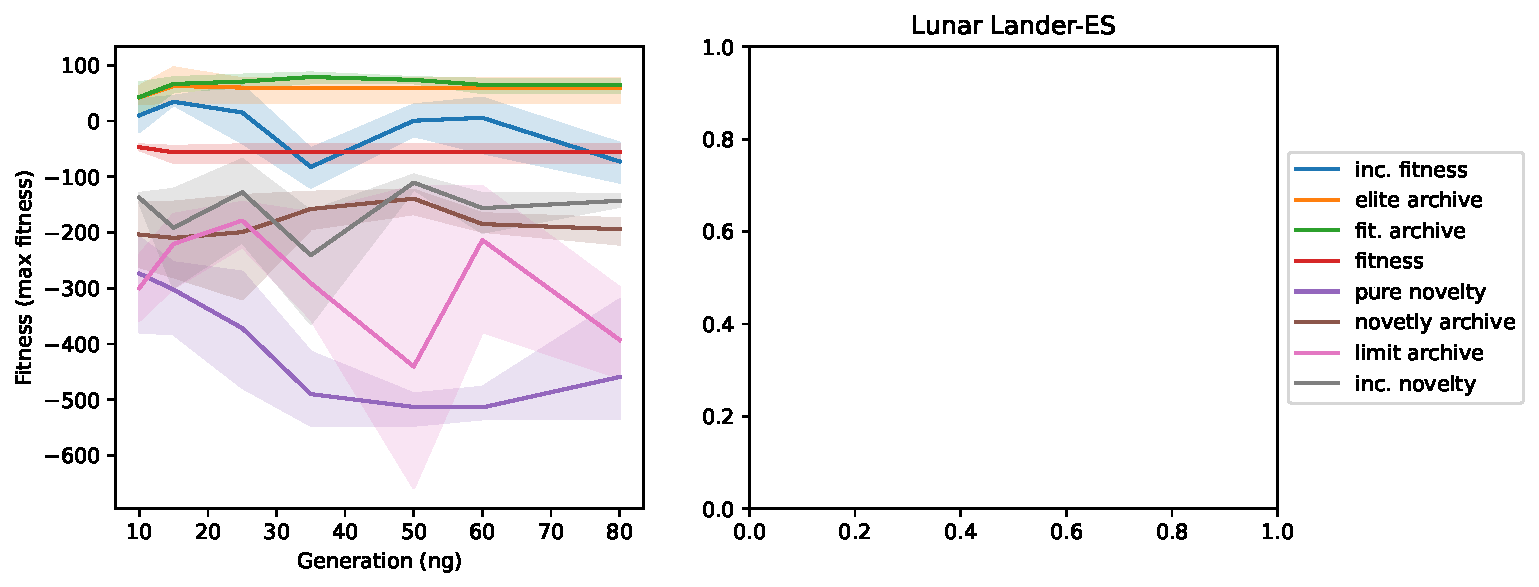
\includegraphics[width=0.8\textwidth]{../img/generations_lunarlander_lambda_max_fit.pdf}
	\caption{Maximal fitness performance characteristic of DE on LL.}
	\label{fig:fitness1}
\end{figure}
\begin{figure}[ht]
	\centering
	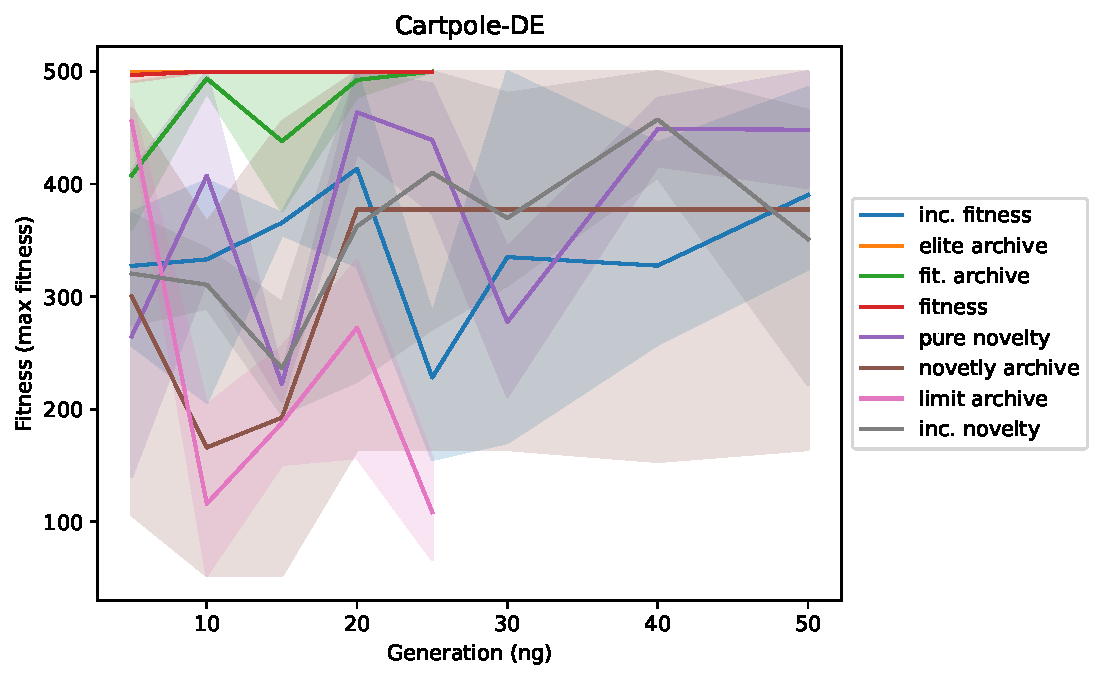
\includegraphics[width=0.8\textwidth]{../img/generations_cartpole_diff_max_fit.pdf}
	\caption{Maximal fitness performance characteristic of DE in Cartpole environment.}
	\label{fig:fitness2}
\end{figure}

\begin{figure}[ht]
	\centering
	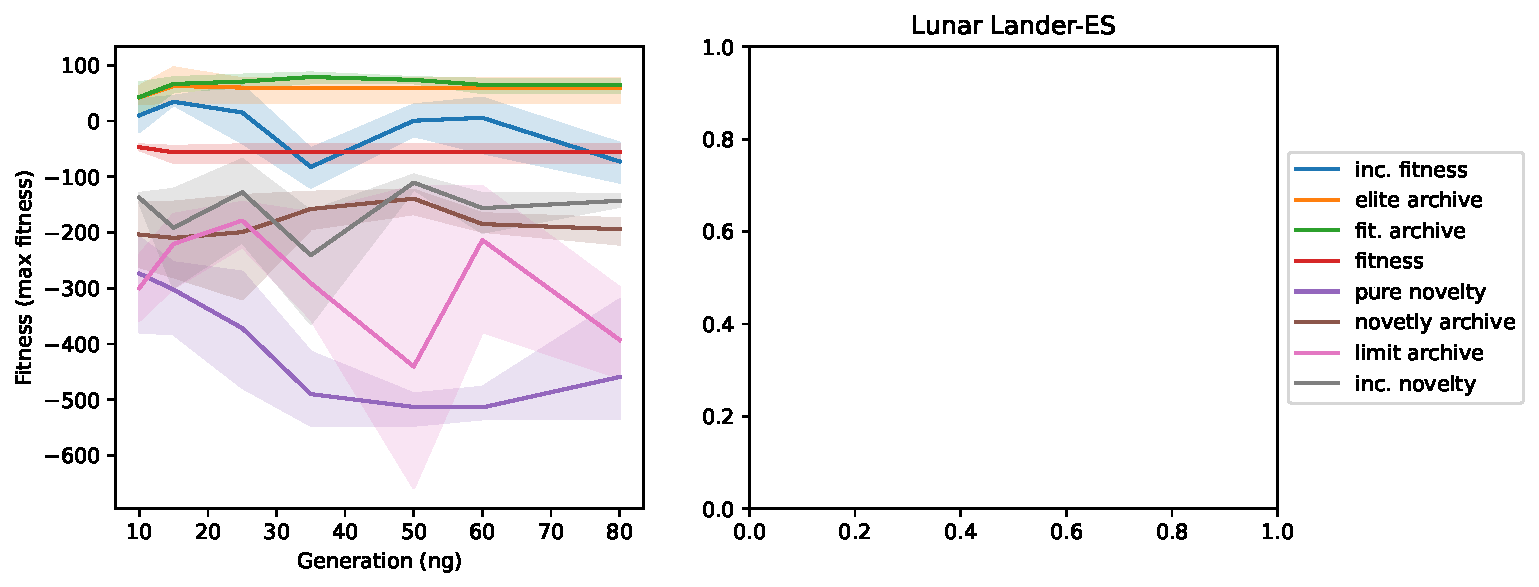
\includegraphics[width=0.8\textwidth]{../img/generations_lunarlander_lambda_max_fit.pdf}
	\caption{Maximal fitness performance characteristic of ES on LL.}
	\label{fig:fitness3}
\end{figure}
\begin{figure}[ht]
	\centering
	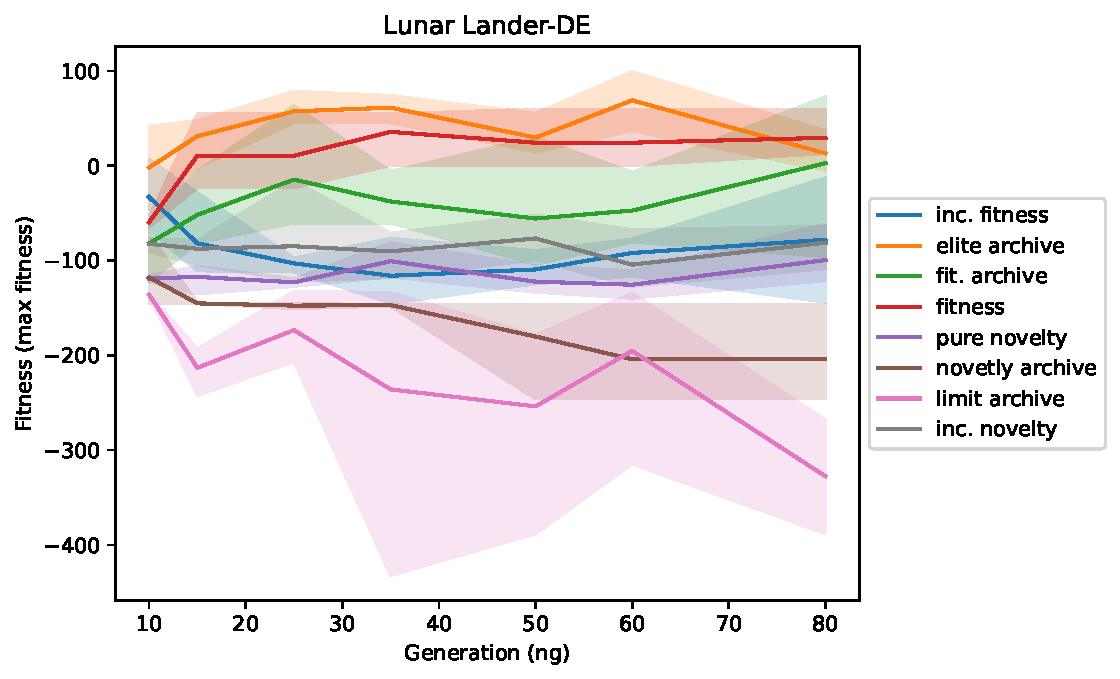
\includegraphics[width=0.8\textwidth]{../img/generations_lunarlander_diff_max_fit.pdf}
	\caption{Maximal fitness performance characteristic of DE on LL.}
	\label{fig:fitness4}
\end{figure}

\Crefrange{fig:fitness1}{fig:fitness4} however have been pruned for readability and do not represent the full range of values that have been taken into account such as the population median or mean. The shaded area represents quantiles $ q_{75} and q_{25} $ other values have been pruned. The actual scope of values considered for each contained is represented by chart that have been for readability sake put into \cref{app:generationGrid}. We evaluated the algorithm on 5 different seeds.

The hand-selected generation counts for the final evaluation are described in \cref{tab:gridResults}.  

\begin{table}[ht]
	\centering
	\scriptsize
	\setlength{\tabcolsep}{4pt}
	\renewcommand{\arraystretch}{1.15}
	\begin{tabular}{l||cc|cc}
		\toprule
		{} & \multicolumn{2}{l}{Lunar Lander} & \multicolumn{2}{l}{Cartpole} \\
		{} &           DE &  ES &       DE &  ES \\
		\midrule
		fitness         &           35 &  25 &       15 &  10 \\
		pure novelty    &           15 &  10 &       25 &  40 \\
		fit. archive    &           80 &  15 &       35 &  25 \\
		inc. fitness    &           15 &  15 &       15 &  20 \\
		inc. novelty    &           25 &  25 &       20 &  40 \\
		novetly archive &           25 &  60 &       20 &  20 \\
		elite archive   &           60 &  15 &       20 &  10 \\
		limit archive   &           25 &  25 &       20 &  20 \\
		\bottomrule
	\end{tabular}
	
	\caption{Selection of generations hyperparameter based on performed grid search}
	\label{tab:gridResults}
\end{table}

\section{Final Results}
After obtaining what we believe to be best performing available hyper-parameters for all containers, we apply this to the final round of tests. We will run the parameterised algorithms on 45 distinct seeds for each environment from which we collect data about the last population. We will subject the colect data to the statistical tests described in section \ref{sec:prefinalComp}. First we will test results of both evolutionary algorithms we have utilised (DE and ES) collected across all containers. Then we will test differences between the objective handling methods. Then we will group these methods based on objective used, following the internal divide in section \ref{sec:objFunc}. Since the groupings of results are different in each case, we claim them to be different test families for the purposes of ajdustments to  \textit{FWER}. 
    
\subsection{EA comparison}
Since we examine only two distinct EA implementations we have directly performed Wilcoxon test. First we see how the EAs performed on each of the environments separately. On both environments the Wilcoxon test rejects the null hypotesis with p values $ p_{LL} = 6.76 \times 10^{-11} $ and $ p_{CT} = 0.0002$ for Lunar lander and Cartpole respectively. On each of the enviroments we calculate the direction of the difference  through Hodges–Lehmann estimator over the differences $  d_i = ES_i - DE_i $. 
Directional values are $ HL_{LL} = -68.8 $ and $ HL_{CT} = 29.12 $ suggesting that DE has been more performant on Lunar lander while ES has been more performant on Cartpole.
Finally we pool the run from both environments and perform global Wilcox test. Unsuprisingly in the pooled cased we do not find enough evidence to reject $ H_0 $ ($ W_T = 60862$, $ p = 0.224$) as the per-environment performances largely cancel out. 
\subsection{Objective handling comparison}
Now we want to compare the objective handling methods based on fitness of individuals they have produced.
Friedman test rejects the null hypotesis for both Lunar Lander ($ \chi_F = 210.29 $, $ p_F = 7.57 \times 10^{-42} $) and Cartpole ($ \chi_F = 326.66 $, $ p_F = 1.21 \times 10^{-66} $). So we proceed to the pairwise Wilcoxon tests on both environments. The results are shown in \cref{tab:contWilcoxonLL,tab:contWilcoxonCT} respectively.

\begin{table}[ht]
	\centering
	\scriptsize
	\setlength{\tabcolsep}{4pt}
	\renewcommand{\arraystretch}{1.15}
	\resizebox{\textwidth}{!}{%
	\begin{tabular}{cc||ccccccc}
		\toprule
		A &               B &   $W_T$ &                     p &          HL &            $p_{Holm}$ &            $p_{Hoch}$ & Conclusion \\
		\midrule
		fitness &    pure novelty & 170.000 &  $4.15\times 10^{-8}$ &  128.843167 &  $6.22\times 10^{-7}$ &  $6.22\times 10^{-7}$ &   rejected \\
		fitness &    inc. fitness & 873.000 &                 0.928 &           - &                 1.000 &                 0.928 &  sustained \\
		fitness &    inc. novelty & 226.000 &  $3.93\times 10^{-7}$ &   92.643877 &  $4.72\times 10^{-6}$ &  $4.72\times 10^{-6}$ &   rejected \\
		fitness &    fit. archive & 765.000 &                 0.269 &           - &                 0.808 &                 0.808 &  sustained \\
		fitness &   elite archive & 686.000 &                 0.092 &           - &                 0.633 &                 0.434 &  sustained \\
		fitness & novetly archive &  71.000 & $5.19\times 10^{-10}$ &  139.303538 &  $1.04\times 10^{-8}$ &  $1.04\times 10^{-8}$ &   rejected \\
		fitness &   limit archive &  68.000 & $4.51\times 10^{-10}$ &  224.407512 &  $1.04\times 10^{-8}$ &  $1.04\times 10^{-8}$ &   rejected \\
		pure novelty &    inc. fitness & 149.000 &  $1.71\times 10^{-8}$ & -114.614712 &  $2.91\times 10^{-7}$ &  $2.91\times 10^{-7}$ &   rejected \\
		pure novelty &    inc. novelty & 685.000 &                 0.090 &           - &                 0.633 &                 0.434 &  sustained \\
		pure novelty &    fit. archive &  60.000 & $3.09\times 10^{-10}$ & -129.703835 &  $7.42\times 10^{-9}$ &  $7.42\times 10^{-9}$ &   rejected \\
		pure novelty &   elite archive &  70.000 & $4.95\times 10^{-10}$ & -147.305362 &  $1.04\times 10^{-8}$ &  $1.04\times 10^{-8}$ &   rejected \\
		pure novelty & novetly archive & 697.000 &                 0.109 &           - &                 0.633 &                 0.434 &  sustained \\
		pure novelty &   limit archive & 320.000 &  $1.19\times 10^{-5}$ &   91.802822 &  $1.30\times 10^{-4}$ &  $1.30\times 10^{-4}$ &   rejected \\
		inc. fitness &    inc. novelty & 190.000 &  $9.44\times 10^{-8}$ &   92.265044 &  $1.32\times 10^{-6}$ &  $1.32\times 10^{-6}$ &   rejected \\
		inc. fitness &    fit. archive & 686.000 &                 0.092 &           - &                 0.633 &                 0.434 &  sustained \\
		inc. fitness &   elite archive & 646.000 &                 0.048 &           - &                 0.381 &                 0.381 &  sustained \\
		inc. fitness & novetly archive &  69.000 & $4.73\times 10^{-10}$ &  145.000351 &  $1.04\times 10^{-8}$ &  $1.04\times 10^{-8}$ &   rejected \\
		inc. fitness &   limit archive &   9.000 & $2.56\times 10^{-11}$ &  227.153914 & $7.18\times 10^{-10}$ & $7.18\times 10^{-10}$ &   rejected \\
		inc. novelty &    fit. archive &  87.000 &  $1.09\times 10^{-9}$ & -108.043891 &  $1.96\times 10^{-8}$ &  $1.96\times 10^{-8}$ &   rejected \\
		inc. novelty &   elite archive & 165.000 &  $3.37\times 10^{-8}$ & -128.079075 &  $5.39\times 10^{-7}$ &  $5.39\times 10^{-7}$ &   rejected \\
		inc. novelty & novetly archive & 437.000 &  $4.33\times 10^{-4}$ &   39.747988 &                 0.004 &                 0.004 &   rejected \\
		inc. novelty &   limit archive & 196.000 &  $1.20\times 10^{-7}$ &  120.348414 &  $1.56\times 10^{-6}$ &  $1.56\times 10^{-6}$ &   rejected \\
		fit. archive &   elite archive & 837.000 &                 0.566 &           - &                 1.000 &                 0.928 &  sustained \\
		fit. archive & novetly archive &  54.000 & $2.32\times 10^{-10}$ &  159.409308 &  $5.81\times 10^{-9}$ &  $5.81\times 10^{-9}$ &   rejected \\
		fit. archive &   limit archive &  15.000 & $3.46\times 10^{-11}$ &  244.356882 & $9.35\times 10^{-10}$ & $9.35\times 10^{-10}$ &   rejected \\
		elite archive & novetly archive &  74.000 & $5.97\times 10^{-10}$ &   168.11856 &  $1.14\times 10^{-8}$ &  $1.14\times 10^{-8}$ &   rejected \\
		elite archive &   limit archive &  28.000 & $6.59\times 10^{-11}$ &  248.159355 &  $1.71\times 10^{-9}$ &  $1.71\times 10^{-9}$ &   rejected \\
		novetly archive &   limit archive & 396.000 &  $1.33\times 10^{-4}$ &   77.327852 &                 0.001 &                 0.001 &   rejected \\
		\bottomrule
	\end{tabular}
	}	
	\caption{Fitness Wilcoxon test over objectives handlers for Lunar Lander}
	\label{tab:contWilcoxonLL}
\end{table}

\begin{table}[ht]
	\centering
	\scriptsize
	\setlength{\tabcolsep}{4pt}
	\renewcommand{\arraystretch}{1.15}
	\resizebox{\textwidth}{!}{%
\begin{tabular}{cc||ccccccc}
	\toprule
	A &               B &    $W_T$ &                     p &          HL &            $p_{Holm}$ &            $p_{Hoch}$ & Conclusion \\
	\midrule
	fitness &    pure novelty &   50.000 & $3.85\times 10^{-13}$ &  179.666667 & $6.54\times 10^{-12}$ & $6.54\times 10^{-12}$ &   rejected \\
	fitness &    inc. fitness &  198.500 &  $2.20\times 10^{-7}$ &   79.916667 &  $2.86\times 10^{-6}$ &  $2.86\times 10^{-6}$ &   rejected \\
	fitness &    inc. novelty &   66.000 & $4.01\times 10^{-14}$ &  195.416667 & $8.41\times 10^{-13}$ & $8.41\times 10^{-13}$ &   rejected \\
	fitness &    fit. archive &  324.000 &                 0.111 &           - &                 0.444 &                 0.444 &  sustained \\
	fitness &   elite archive &  138.500 &                 0.088 &           - &                 0.438 &                 0.438 &  sustained \\
	fitness & novetly archive &   11.000 & $1.73\times 10^{-15}$ &       287.5 & $4.66\times 10^{-14}$ & $4.66\times 10^{-14}$ &   rejected \\
	fitness &   limit archive &   70.000 & $2.03\times 10^{-14}$ &  212.666667 & $4.47\times 10^{-13}$ & $4.47\times 10^{-13}$ &   rejected \\
	pure novelty &    inc. fitness &  987.000 &  $2.31\times 10^{-4}$ &      -97.25 &                 0.002 &                 0.002 &   rejected \\
	pure novelty &    inc. novelty & 1553.000 &                 0.229 &           - &                 0.687 &                 0.604 &  sustained \\
	pure novelty &    fit. archive &  118.000 & $2.15\times 10^{-12}$ & -168.083333 & $3.43\times 10^{-11}$ & $3.43\times 10^{-11}$ &   rejected \\
	pure novelty &   elite archive &   34.000 & $1.38\times 10^{-13}$ & -190.083333 & $2.48\times 10^{-12}$ & $2.48\times 10^{-12}$ &   rejected \\
	pure novelty & novetly archive & 1149.500 &  $3.02\times 10^{-4}$ &  108.416667 &                 0.003 &                 0.002 &   rejected \\
	pure novelty &   limit archive & 1710.000 &                 0.302 &           - &                 0.687 &                 0.604 &  sustained \\
	inc. fitness &    inc. novelty &  733.500 &  $2.74\times 10^{-6}$ &       110.5 &  $3.29\times 10^{-5}$ &  $3.29\times 10^{-5}$ &   rejected \\
	inc. fitness &    fit. archive &  444.000 &  $8.41\times 10^{-6}$ &  -63.416667 &  $9.25\times 10^{-5}$ &  $9.25\times 10^{-5}$ &   rejected \\
	inc. fitness &   elite archive &   27.000 & $3.19\times 10^{-10}$ &  -86.083333 &  $4.79\times 10^{-9}$ &  $4.79\times 10^{-9}$ &   rejected \\
	inc. fitness & novetly archive &  149.000 & $8.01\times 10^{-14}$ &  200.333333 & $1.52\times 10^{-12}$ & $1.52\times 10^{-12}$ &   rejected \\
	inc. fitness &   limit archive &  520.000 &  $2.19\times 10^{-9}$ &  128.083333 &  $3.06\times 10^{-8}$ &  $3.06\times 10^{-8}$ &   rejected \\
	inc. novelty &    fit. archive &   44.000 & $6.07\times 10^{-14}$ &      -182.5 & $1.21\times 10^{-12}$ & $1.21\times 10^{-12}$ &   rejected \\
	inc. novelty &   elite archive &   16.000 & $1.43\times 10^{-14}$ & -204.333333 & $3.44\times 10^{-13}$ & $3.44\times 10^{-13}$ &   rejected \\
	inc. novelty & novetly archive & 1115.000 &  $2.82\times 10^{-4}$ &   87.416667 &                 0.003 &                 0.002 &   rejected \\
	inc. novelty &   limit archive & 1930.000 &                 0.636 &           - &                 0.687 &                 0.636 &  sustained \\
	fit. archive &   elite archive &  134.000 &                 0.001 &         0.0 &                 0.006 &                 0.006 &   rejected \\
	fit. archive & novetly archive &   18.000 & $2.21\times 10^{-15}$ &  276.083333 & $5.75\times 10^{-14}$ & $5.75\times 10^{-14}$ &   rejected \\
	fit. archive &   limit archive &   86.000 & $1.54\times 10^{-14}$ &       198.5 & $3.54\times 10^{-13}$ & $3.54\times 10^{-13}$ &   rejected \\
	elite archive & novetly archive &    5.000 & $1.39\times 10^{-15}$ &  302.833333 & $3.90\times 10^{-14}$ & $3.90\times 10^{-14}$ &   rejected \\
	elite archive &   limit archive &   27.000 & $3.04\times 10^{-15}$ &  220.833333 & $7.59\times 10^{-14}$ & $7.59\times 10^{-14}$ &   rejected \\
	novetly archive &   limit archive & 1164.000 &  $3.78\times 10^{-4}$ &  -68.416667 &                 0.003 &                 0.003 &   rejected \\
	\bottomrule
\end{tabular}
}
	\caption{Fitness Wilcoxon test over objectives handlers for Cartpole}
	\label{tab:contWilcoxonCT}
\end{table}
\subsection{Diversity Comparison}
Now that we have made the comparison on achieved fitness we want to compare the algorithms also based on the produced diversity.
The Friedman test rejects the null hypotesis also for divirsities both for Lunar Lander ($ \chi_F = 192.23 $, $ p_F = 5 \times 10^{-38} $) and Cartpole ($ \chi_F = 163.918 $, $ p_F = 4.8 \times 10^{-32} $) and so we can safely perform Wilcoxon test on the combinations of objective handling methods. Results are shown in \cref{tab:contWilcoxonCTDiv,tab:contWilcoxonLLDiv}.

\begin{table}[ht]
	\centering
	\scriptsize
	\setlength{\tabcolsep}{4pt}
	\renewcommand{\arraystretch}{1.15}
	\resizebox{\textwidth}{!}{%
		\begin{tabular}{lcccccccc}
			\toprule
			A &               B &   $W_T$ &                     p &        HL &            $p_{Holm}$ &            $p_{Hoch}$ & Conclusion \\
			\midrule
			fitness &    pure novelty & 1323.00 &                  0.00 & -0.042555 &                  0.04 &                  0.04 &   rejected \\
			fitness &    inc. fitness &  947.00 &  $9.51\times 10^{-6}$ &  0.090809 &  $1.33\times 10^{-4}$ &  $1.33\times 10^{-4}$ &   rejected \\
			fitness &    inc. novelty & 1640.00 &                  0.10 &         - &                  0.51 &                  0.51 &  sustained \\
			fitness &    fit. archive & 1183.00 &  $5.04\times 10^{-4}$ &  0.073376 &                  0.01 &                  0.01 &   rejected \\
			fitness &   elite archive &  189.00 & $7.54\times 10^{-14}$ &  0.217708 & $2.04\times 10^{-12}$ & $2.04\times 10^{-12}$ &   rejected \\
			fitness & novetly archive &  650.00 &  $1.88\times 10^{-8}$ &  0.225698 &  $3.94\times 10^{-7}$ &  $3.94\times 10^{-7}$ &   rejected \\
			fitness &   limit archive &  829.00 &  $9.44\times 10^{-7}$ &  0.146048 &  $1.70\times 10^{-5}$ &  $1.70\times 10^{-5}$ &   rejected \\
			pure novelty &    inc. fitness &  735.00 &  $1.28\times 10^{-7}$ &  0.149859 &  $2.57\times 10^{-6}$ &  $2.57\times 10^{-6}$ &   rejected \\
			pure novelty &    inc. novelty & 1941.00 &                  0.67 &         - &                  1.00 &                  0.84 &  sustained \\
			pure novelty &    fit. archive &  464.00 & $1.87\times 10^{-10}$ &  0.129778 &  $4.31\times 10^{-9}$ &  $4.31\times 10^{-9}$ &   rejected \\
			pure novelty &   elite archive &   45.00 & $7.79\times 10^{-16}$ &  0.262882 & $2.18\times 10^{-14}$ & $2.18\times 10^{-14}$ &   rejected \\
			pure novelty & novetly archive &  271.00 & $8.80\times 10^{-13}$ &  0.272268 & $2.29\times 10^{-11}$ & $2.29\times 10^{-11}$ &   rejected \\
			pure novelty &   limit archive &  393.00 & $2.79\times 10^{-11}$ &   0.19342 & $6.70\times 10^{-10}$ & $6.70\times 10^{-10}$ &   rejected \\
			inc. fitness &    inc. novelty &  930.00 &  $6.91\times 10^{-6}$ & -0.114747 &  $1.04\times 10^{-4}$ &  $1.04\times 10^{-4}$ &   rejected \\
			inc. fitness &    fit. archive & 1804.00 &                  0.33 &         - &                  0.98 &                  0.84 &  sustained \\
			inc. fitness &   elite archive &  959.00 &  $1.19\times 10^{-5}$ &  0.122055 &  $1.54\times 10^{-4}$ &  $1.54\times 10^{-4}$ &   rejected \\
			inc. fitness & novetly archive & 1354.00 &                  0.01 &  0.125952 &                  0.05 &                  0.05 &   rejected \\
			inc. fitness &   limit archive & 1754.00 &                  0.24 &         - &                  0.95 &                  0.84 &  sustained \\
			inc. novelty &    fit. archive &  923.00 &  $6.05\times 10^{-6}$ &  0.111492 &  $9.68\times 10^{-5}$ &  $9.68\times 10^{-5}$ &   rejected \\
			inc. novelty &   elite archive &  283.00 & $1.25\times 10^{-12}$ &  0.243282 & $3.12\times 10^{-11}$ & $3.12\times 10^{-11}$ &   rejected \\
			inc. novelty & novetly archive &  596.00 &  $5.21\times 10^{-9}$ &  0.240971 &  $1.15\times 10^{-7}$ &  $1.15\times 10^{-7}$ &   rejected \\
			inc. novelty &   limit archive &  863.00 &  $1.88\times 10^{-6}$ &  0.171545 &  $3.19\times 10^{-5}$ &  $3.19\times 10^{-5}$ &   rejected \\
			fit. archive &   elite archive &  825.00 &  $8.70\times 10^{-7}$ &  0.137525 &  $1.65\times 10^{-5}$ &  $1.65\times 10^{-5}$ &   rejected \\
			fit. archive & novetly archive &  975.00 &  $1.59\times 10^{-5}$ &  0.141326 &  $1.91\times 10^{-4}$ &  $1.91\times 10^{-4}$ &   rejected \\
			fit. archive &   limit archive & 1502.00 &                  0.03 &         - &                  0.17 &                  0.17 &  sustained \\
			elite archive & novetly archive & 1952.00 &                  0.84 &         - &                  1.00 &                  0.84 &  sustained \\
			elite archive &   limit archive & 1482.00 &                  0.02 &         - &                  0.16 &                  0.16 &  sustained \\
			novetly archive &   limit archive & 1309.00 &                  0.02 &         - &                  0.12 &                  0.12 &  sustained \\
			\bottomrule
		\end{tabular}
	}
	\caption{Diversity Wilcoxon test over objectives handlers for Cartpole}
	\label{tab:contWilcoxonCTDiv}
\end{table}

\begin{table}[ht]
	\centering
	\scriptsize
	\setlength{\tabcolsep}{4pt}
	\renewcommand{\arraystretch}{1.15}
	\resizebox{\textwidth}{!}{%
		\begin{tabular}{lcccccccc}
			\toprule
			A &               B &  $W_T$ &                     p &        HL &            $p_{Holm}$ &            $p_{Hoch}$ & Conclusion \\
			\midrule
			fitness &    pure novelty &  49.00 & $1.83\times 10^{-10}$ & -0.102046 &  $4.20\times 10^{-9}$ &  $4.20\times 10^{-9}$ &   rejected \\
			fitness &    inc. fitness & 119.00 &  $1.18\times 10^{-8}$ & -0.069382 &  $2.60\times 10^{-7}$ &  $2.60\times 10^{-7}$ &   rejected \\
			fitness &    inc. novelty & 122.00 &  $2.18\times 10^{-8}$ & -0.075654 &  $4.57\times 10^{-7}$ &  $4.57\times 10^{-7}$ &   rejected \\
			fitness &    fit. archive & 501.00 &                  0.04 &         - &                  0.26 &                  0.26 &  sustained \\
			fitness &   elite archive &  59.00 &  $1.44\times 10^{-7}$ &  0.066169 &  $2.44\times 10^{-6}$ &  $2.44\times 10^{-6}$ &   rejected \\
			fitness & novetly archive & 273.00 &  $2.29\times 10^{-6}$ & -0.119972 &  $3.43\times 10^{-5}$ &  $3.43\times 10^{-5}$ &   rejected \\
			fitness &   limit archive & 609.00 &                  0.25 &         - &                  1.00 &                  0.71 &  sustained \\
			pure novelty &    inc. fitness & 600.00 &                  0.02 &         - &                  0.18 &                  0.18 &  sustained \\
			pure novelty &    inc. novelty & 709.00 &                  0.13 &         - &                  0.65 &                  0.65 &  sustained \\
			pure novelty &    fit. archive & 383.00 &  $8.99\times 10^{-5}$ &  0.082667 &                  0.00 &                  0.00 &   rejected \\
			pure novelty &   elite archive &      0 & $1.63\times 10^{-11}$ &  0.179489 & $4.56\times 10^{-10}$ & $4.56\times 10^{-10}$ &   rejected \\
			pure novelty & novetly archive & 865.00 &                  0.71 &         - &                  1.00 &                  0.71 &  sustained \\
			pure novelty &   limit archive &  25.00 & $5.68\times 10^{-11}$ &  0.123138 &  $1.53\times 10^{-9}$ &  $1.53\times 10^{-9}$ &   rejected \\
			inc. fitness &    inc. novelty & 778.00 &                  0.42 &         - &                  1.00 &                  0.71 &  sustained \\
			inc. fitness &    fit. archive & 586.00 &                  0.02 &         - &                  0.19 &                  0.19 &  sustained \\
			inc. fitness &   elite archive &  11.00 & $6.22\times 10^{-11}$ &  0.141697 &  $1.55\times 10^{-9}$ &  $1.55\times 10^{-9}$ &   rejected \\
			inc. fitness & novetly archive & 694.00 &                  0.10 &         - &                  0.62 &                  0.62 &  sustained \\
			inc. fitness &   limit archive & 169.00 &  $1.07\times 10^{-7}$ &  0.087411 &  $2.03\times 10^{-6}$ &  $2.03\times 10^{-6}$ &   rejected \\
			inc. novelty &    fit. archive & 505.00 &                  0.00 &  0.059472 &                  0.05 &                  0.05 &   rejected \\
			inc. novelty &   elite archive &   1.00 & $7.97\times 10^{-11}$ &  0.148144 &  $1.91\times 10^{-9}$ &  $1.91\times 10^{-9}$ &   rejected \\
			inc. novelty & novetly archive & 809.00 &                  0.44 &         - &                  1.00 &                  0.71 &  sustained \\
			inc. novelty &   limit archive & 197.00 &  $3.43\times 10^{-7}$ &  0.099544 &  $5.48\times 10^{-6}$ &  $5.48\times 10^{-6}$ &   rejected \\
			fit. archive &   elite archive & 125.00 &  $2.50\times 10^{-8}$ &  0.102542 &  $4.99\times 10^{-7}$ &  $4.99\times 10^{-7}$ &   rejected \\
			fit. archive & novetly archive & 358.00 &  $4.12\times 10^{-5}$ & -0.078927 &  $5.36\times 10^{-4}$ &  $5.36\times 10^{-4}$ &   rejected \\
			fit. archive &   limit archive & 491.00 &                  0.00 &  0.052381 &                  0.05 &                  0.05 &   rejected \\
			elite archive & novetly archive &  26.00 & $5.97\times 10^{-11}$ & -0.188639 &  $1.55\times 10^{-9}$ &  $1.55\times 10^{-9}$ &   rejected \\
			elite archive &   limit archive & 181.00 &  $1.77\times 10^{-5}$ & -0.048803 &  $2.48\times 10^{-4}$ &  $2.48\times 10^{-4}$ &   rejected \\
			novetly archive &   limit archive & 198.00 &  $1.30\times 10^{-7}$ &  0.134406 &  $2.35\times 10^{-6}$ &  $2.35\times 10^{-6}$ &   rejected \\
			\bottomrule
		\end{tabular}
	}
	\caption{Diversity Wilcoxon test over objectives handlers for Lunar Lander}
	\label{tab:contWilcoxonLLDiv}
\end{table}
\subsection{Group comparison}
We woul also like to compare the groups based on objective as such (fitness, novelty, combination). For that we wan to assess the group cohesion in each of th 
\section{Discussion}

\chapter*{Conclusion}
\addcontentsline{toc}{chapter}{Conclusion}
I have successfully developed and implemented framework for testing evolutionary strategies and differential evolution in several setups, such as fitness, novelty and their respective archivng and a combination of them. I have also proposed behavioral models for both environments Lunar Lander and Cartpole. These behavioral models are a modest success, while Lunar Lander model, unlike Cartpole, does not consistently achieve solution grade score, it is still very well-behaved. I have also proposed a hyperparameter searching algorithm based on Bayesian search. While the search itself is rather limited, this reflects the conditions of the used environments, which are time-exhausting to simulate in large numbers. The algorithm allows us to compare the EAs on their performance given hyperparameters found by this search.
The areas of comparisons were: absolute performance, rate of convergance and diversity of the final populations.

%%% Bibliography
\include{bibliography}

%%% Figures used in the thesis (consider if this is needed)
\listoffigures

%%% Tables used in the thesis (consider if this is needed)
%%% In mathematical theses, it could be better to move the list of tables to the beginning of the thesis.
\listoftables

%%% Abbreviations used in the thesis, if any, including their explanation
%%% In mathematical theses, it could be better to move the list of abbreviations to the beginning of the thesis.
\chapwithtoc{List of Abbreviations}
\begin{tabular}{ll}
	EA & Evolutionary Algorithm \\
	ES & Evolutionary Strategy \\
	DE & Differential Evolution \\
	BS & Bayesian Search \\
	IGS & Incremental grid search
\end{tabular}



%%% Attachments to the master thesis, if any. Each attachment must be
%%% referred to at least once from the text of the thesis. Attachments
%%% are numbered.
%%%
%%% The printed version should preferably contain attachments, which can be
%%% read (additional tables and charts, supplementary text, examples of
%%% program output, etc.). The electronic version is more suited for attachments
%%% which will likely be used in an electronic form rather than read (program
%%% source code, data files, interactive charts, etc.). Electronic attachments
%%% should be uploaded to SIS and optionally also included in the thesis on a~CD/DVD.
%%% Allowed file formats are specified in provision of the rector no. 72/2017.
\appendix
\chapter{Attachments}
\section{Full grid search charts}
\label{app:generationGrid}

            \begin{figure}[H]
            \centering
            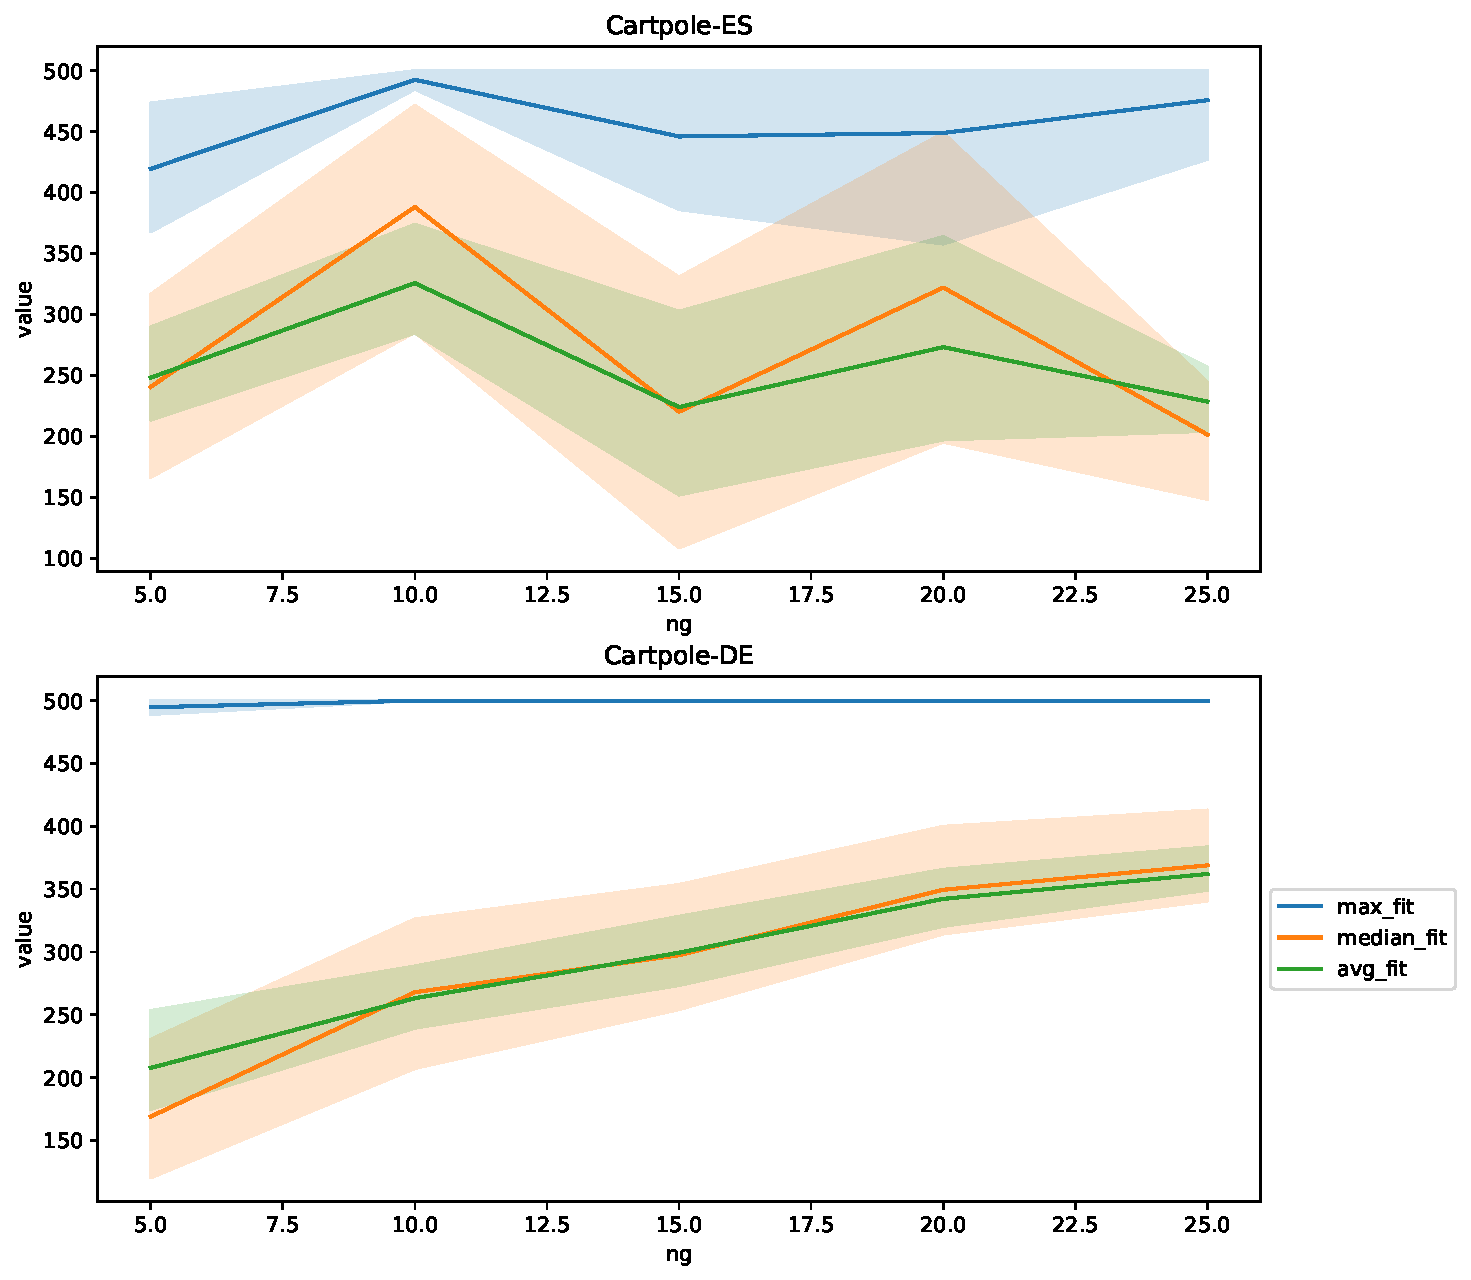
\includegraphics[width=0.9\textwidth]{../img/Origin_generations_cartpole_fitness}
            \caption{Detailed fitness/generation characteristic for fitness on Cartpole env. }
            \label{fig:og_gen_cartpole_fitness}
            \end{figure}

        
            \begin{figure}[H]
            \centering
            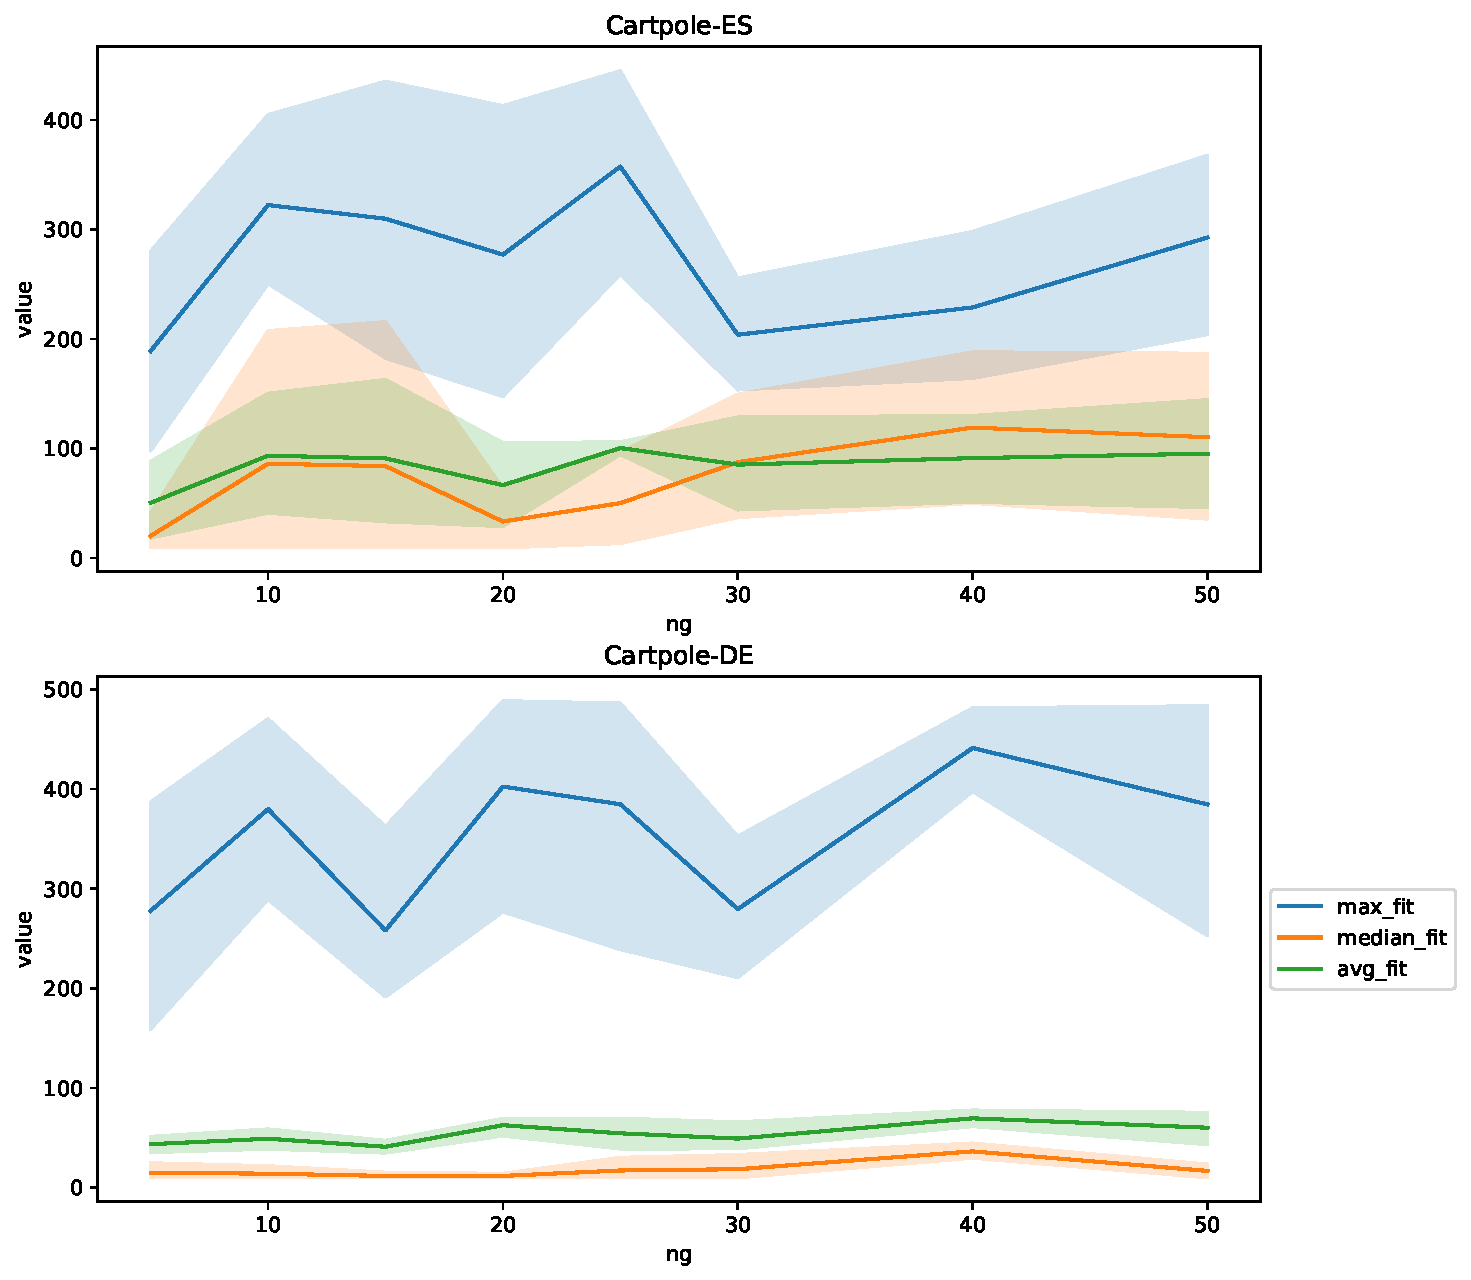
\includegraphics[width=0.9\textwidth]{../img/Origin_generations_cartpole_novelty}
            \caption{Detailed fitness/generation characteristic for pure novelty on Cartpole env. }
            \label{fig:og_gen_cartpole_novelty}
            \end{figure}

        
            \begin{figure}[H]
            \centering
            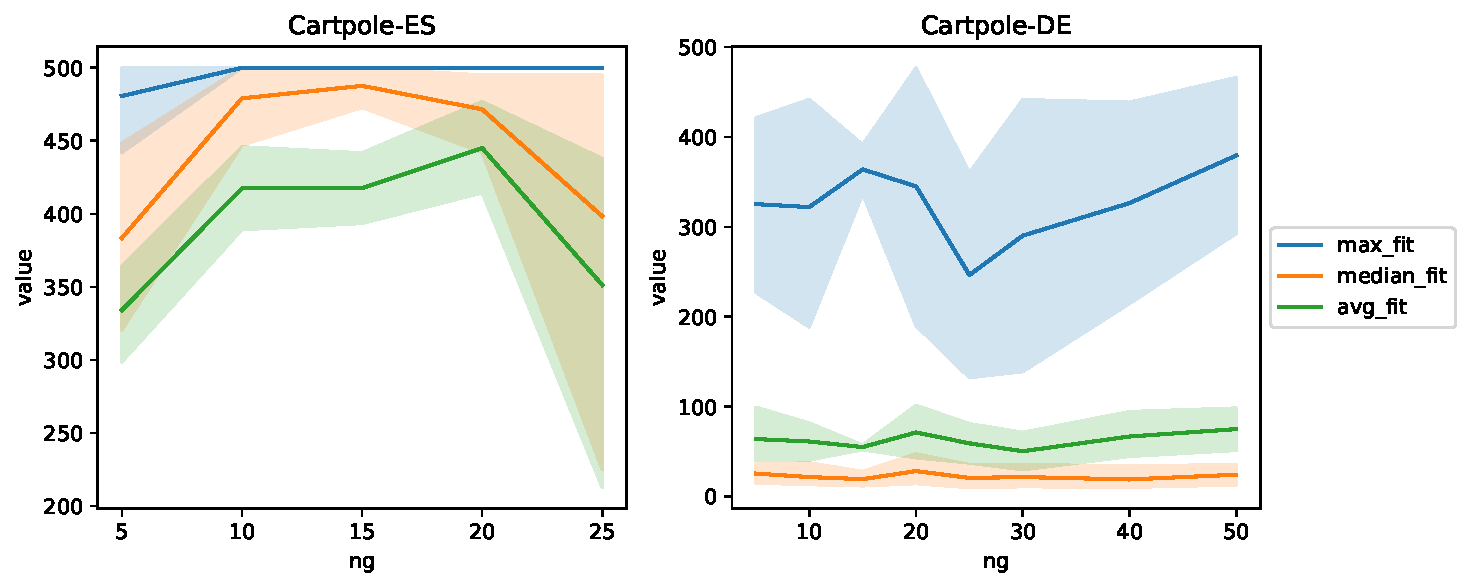
\includegraphics[width=0.9\textwidth]{../img/Origin_generations_cartpole_add_novelty}
            \caption{Detailed fitness/generation characteristic for inc. fitness on Cartpole env. }
            \label{fig:og_gen_cartpole_add_novelty}
            \end{figure}

        
            \begin{figure}[H]
            \centering
            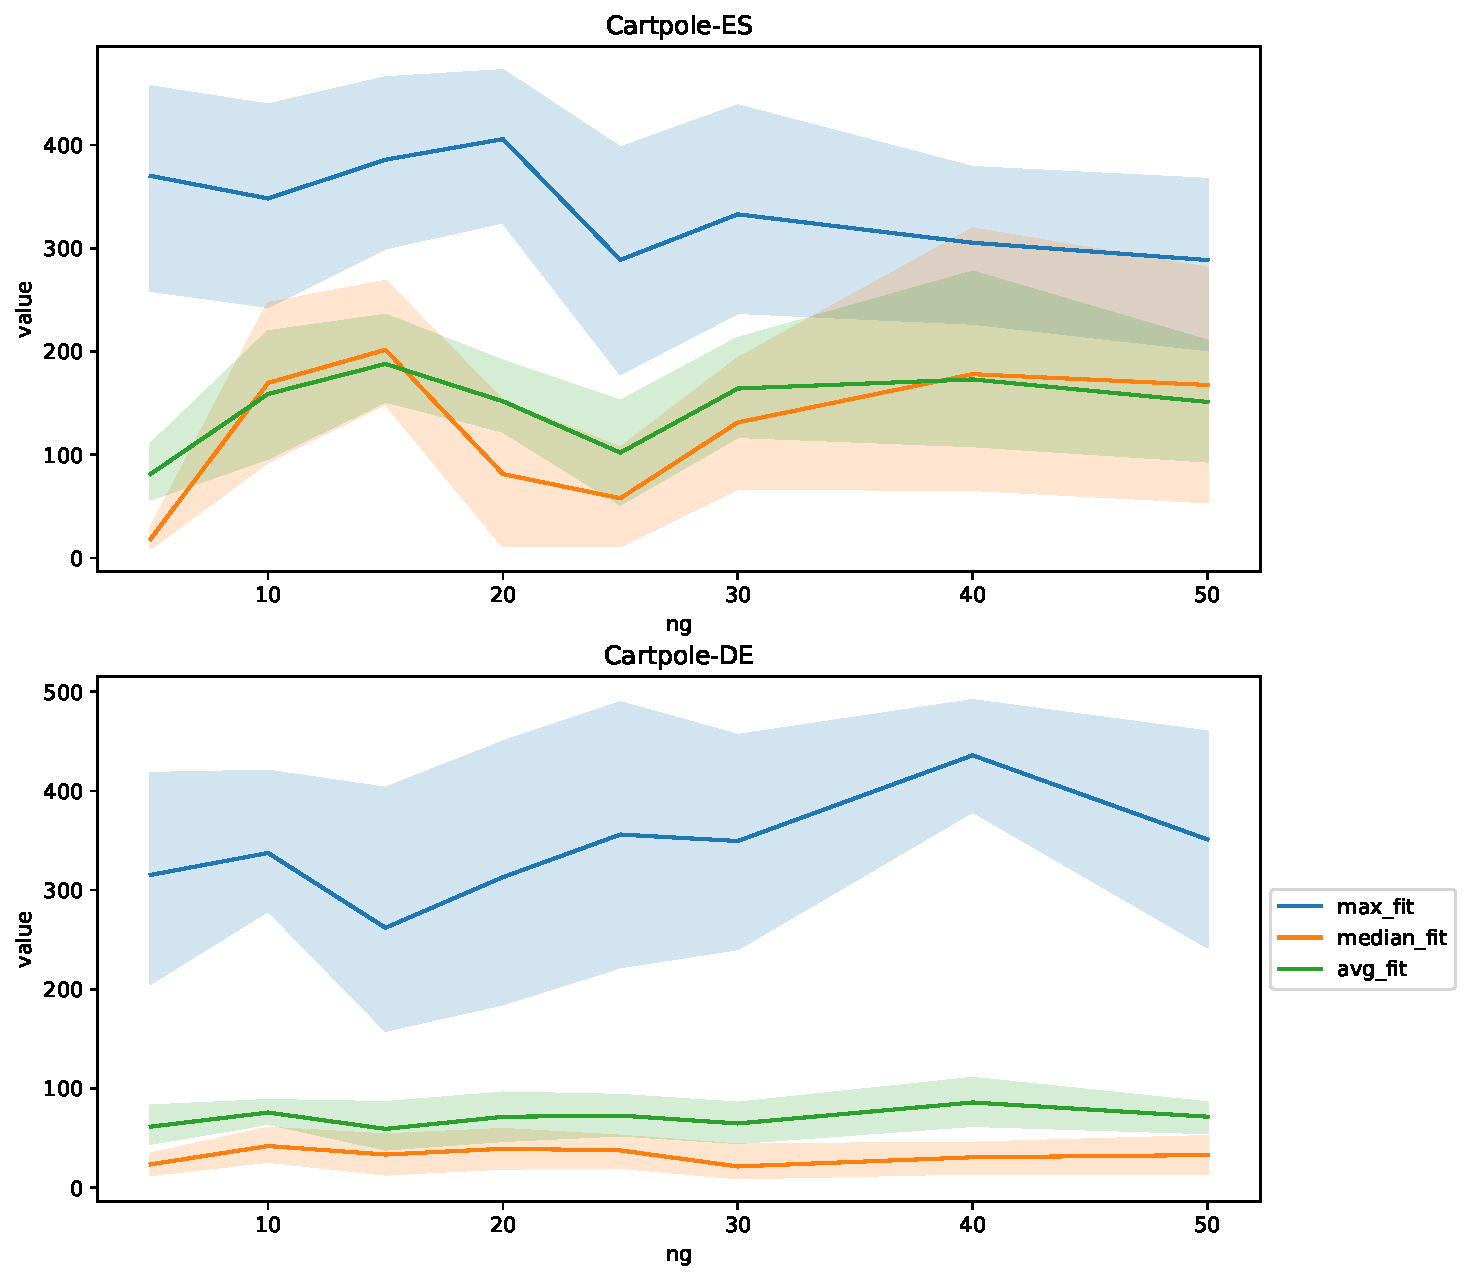
\includegraphics[width=0.9\textwidth]{../img/Origin_generations_cartpole_sub_novelty}
            \caption{Detailed fitness/generation characteristic for inc. novelty on Cartpole env. }
            \label{fig:og_gen_cartpole_sub_novelty}
            \end{figure}

        
            \begin{figure}[H]
            \centering
            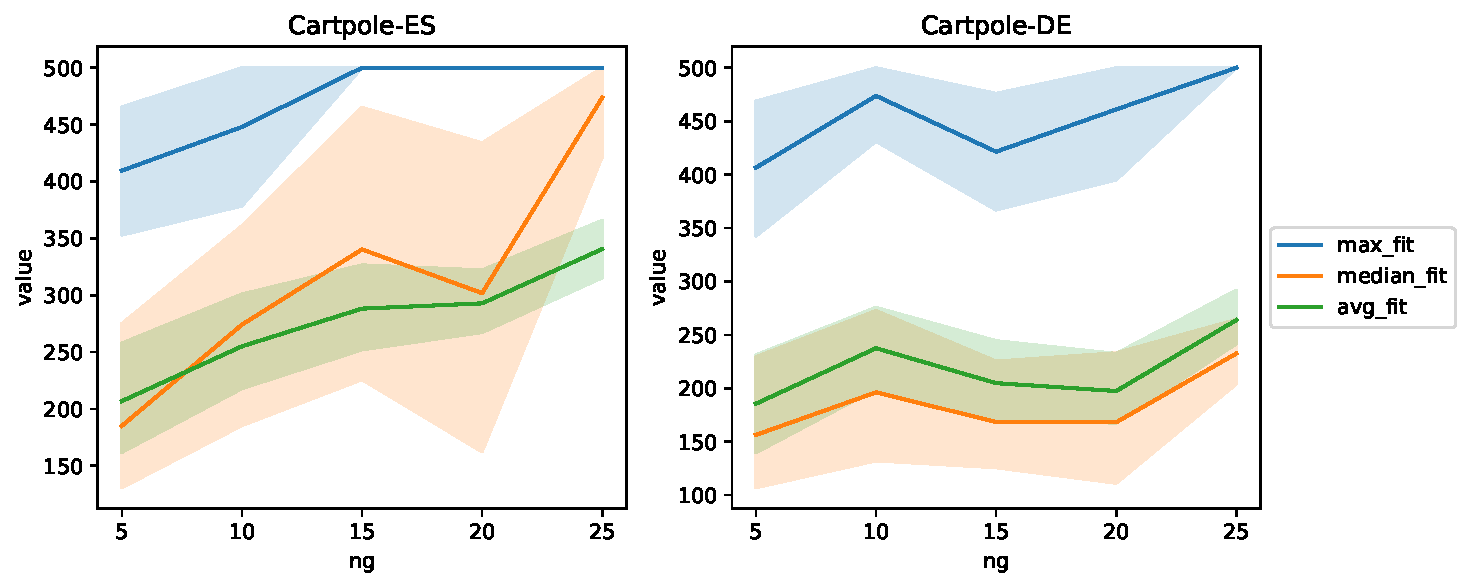
\includegraphics[width=0.9\textwidth]{../img/Origin_generations_cartpole_fit_archiving}
            \caption{Detailed fitness/generation characteristic for fit. archive on Cartpole env. }
            \label{fig:og_gen_cartpole_fit_archiving}
            \end{figure}

        
            \begin{figure}[H]
            \centering
            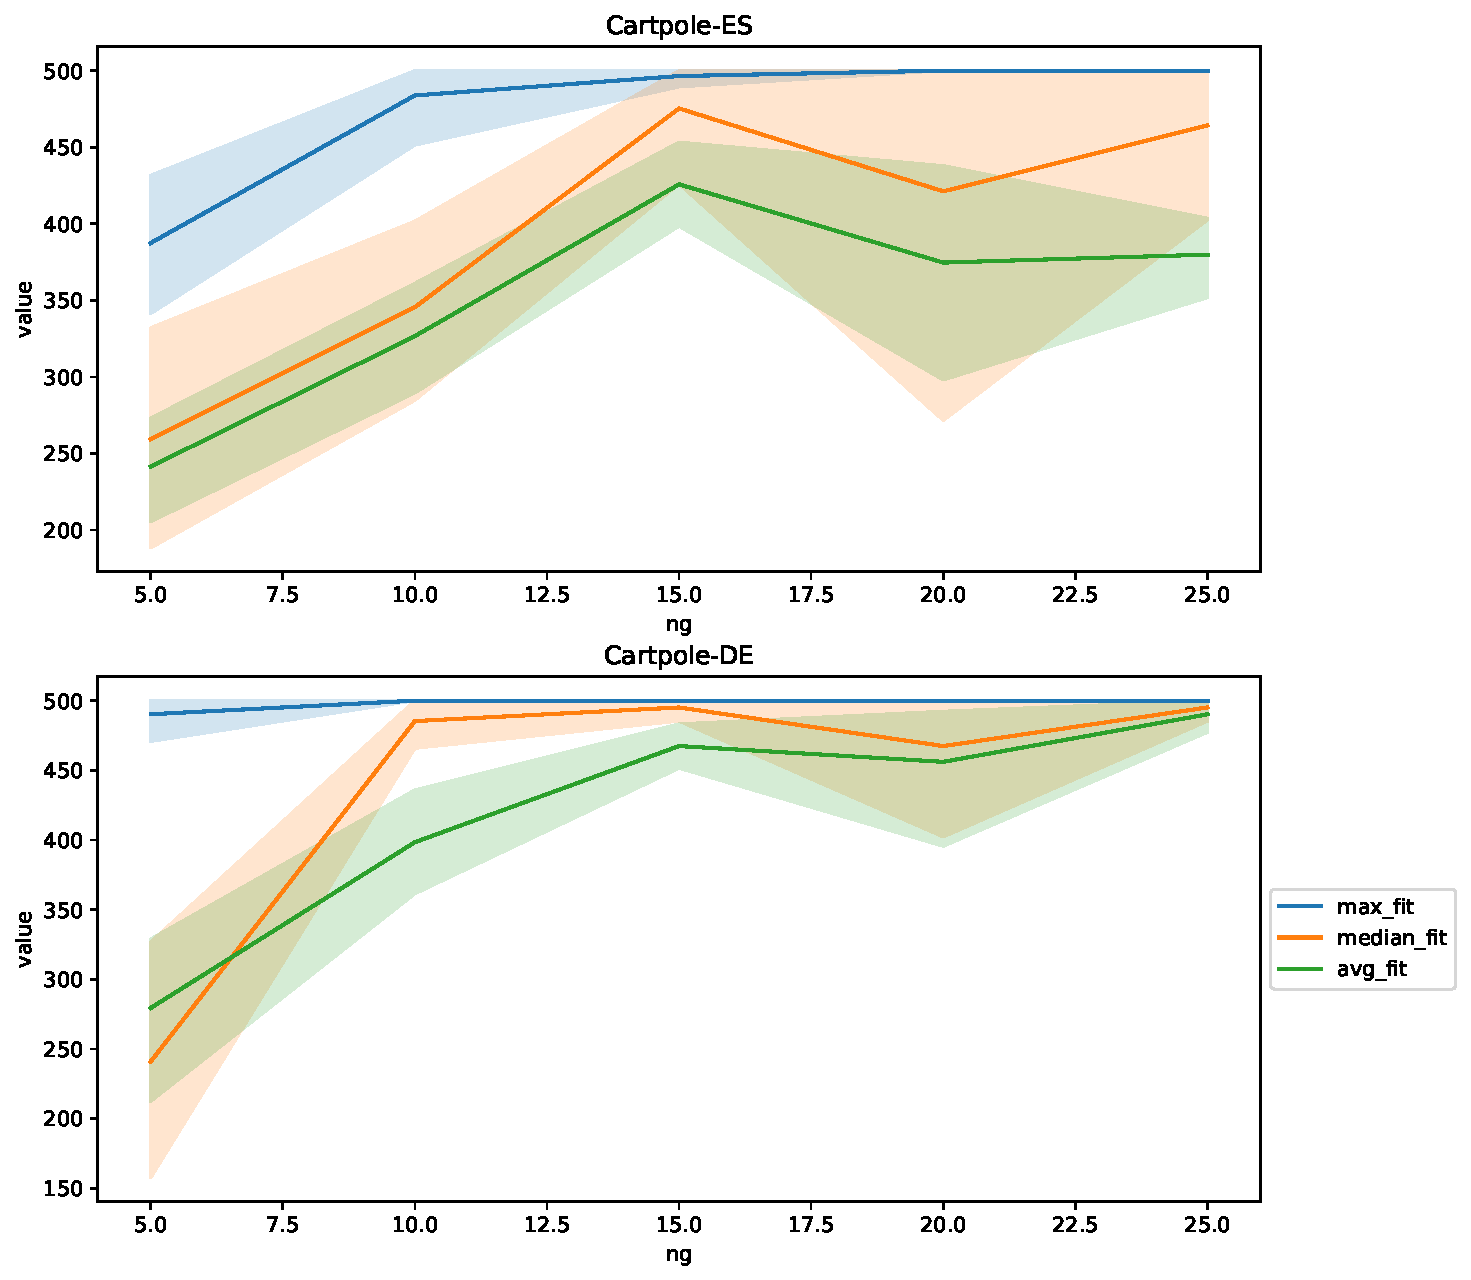
\includegraphics[width=0.9\textwidth]{../img/Origin_generations_cartpole_elite_archiving}
            \caption{Detailed fitness/generation characteristic for elite archive on Cartpole env. }
            \label{fig:og_gen_cartpole_elite_archiving}
            \end{figure}

        
            \begin{figure}[H]
            \centering
            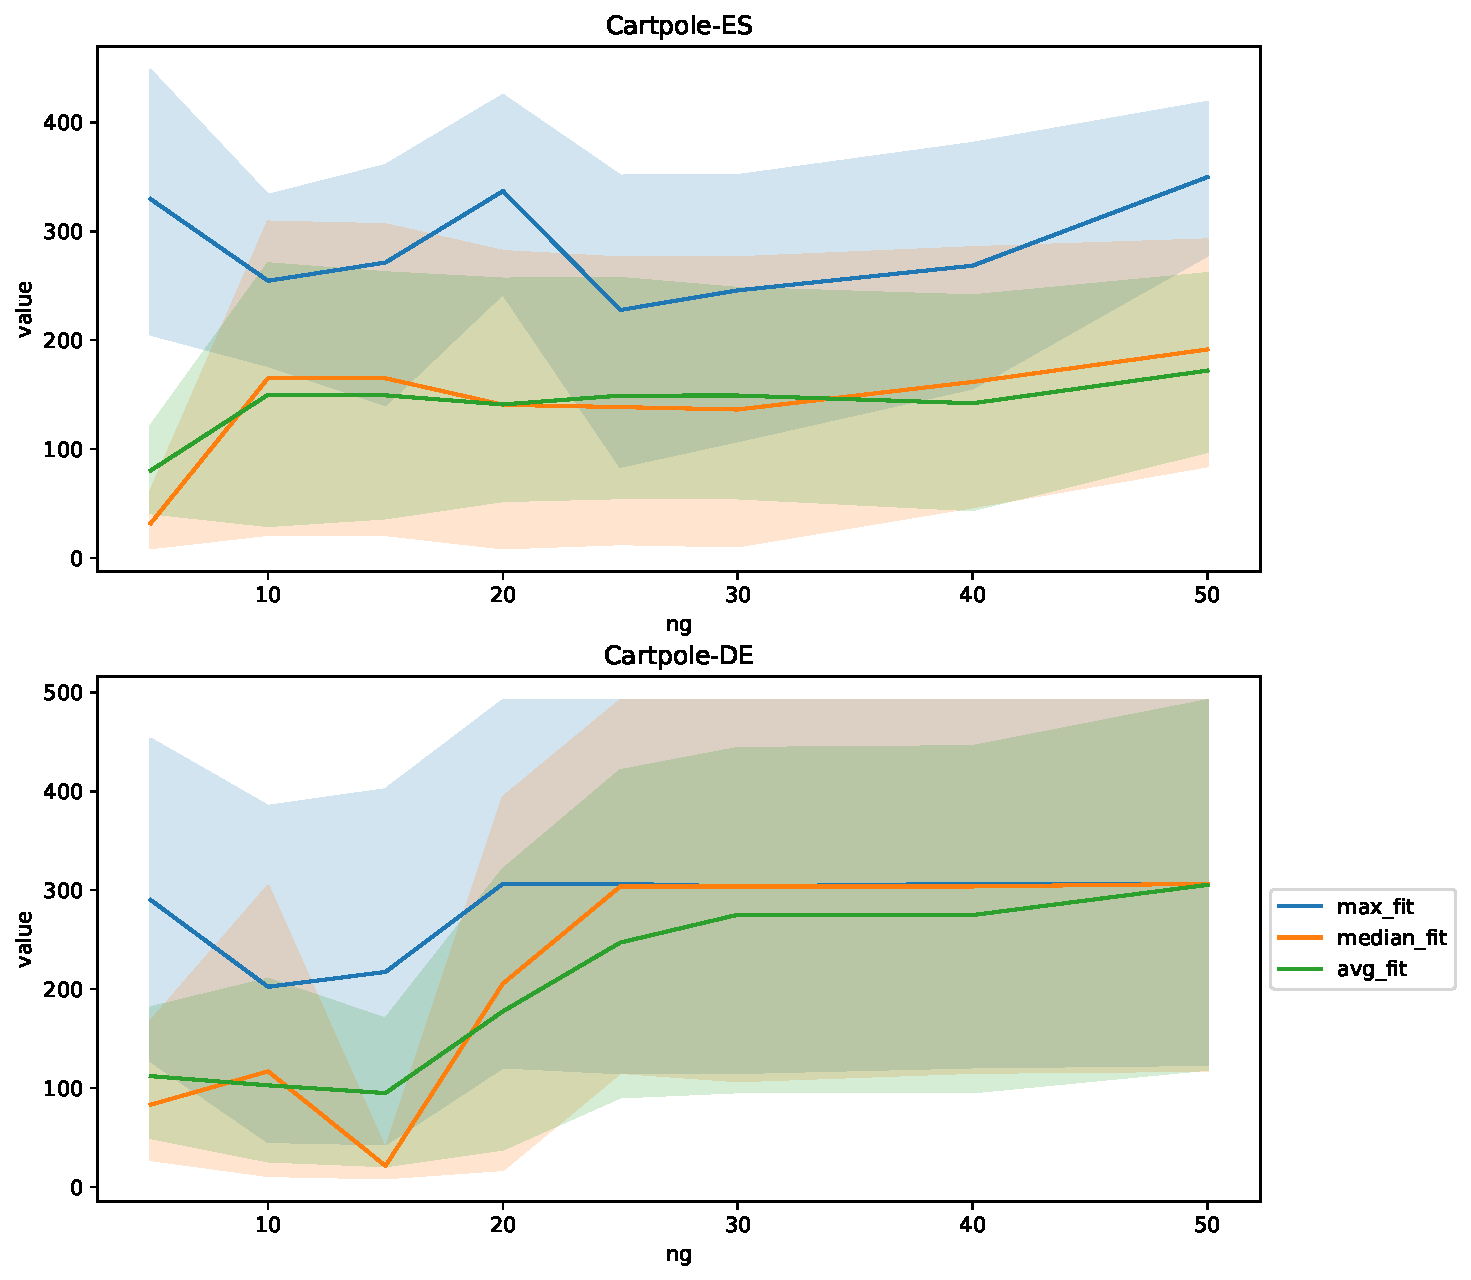
\includegraphics[width=0.9\textwidth]{../img/Origin_generations_cartpole_novelty_archiving}
            \caption{Detailed fitness/generation characteristic for novelty archive on Cartpole env. }
            \label{fig:og_gen_cartpole_novelty_archiving}
            \end{figure}

        
            \begin{figure}[H]
            \centering
            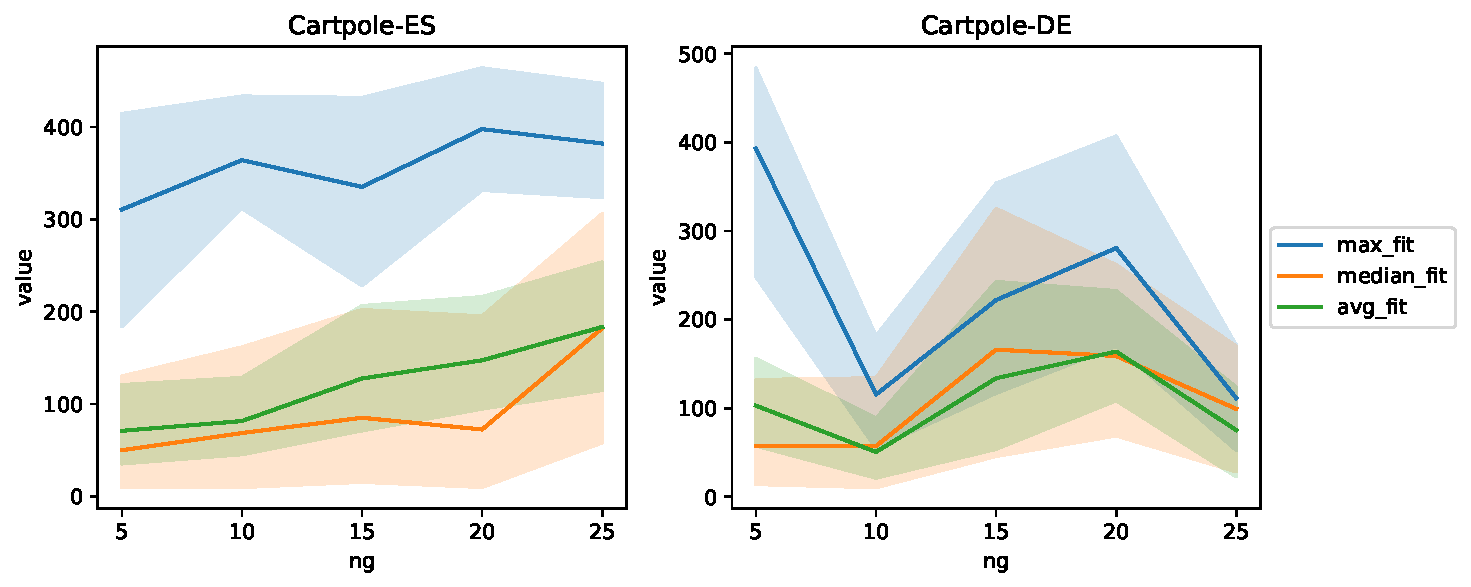
\includegraphics[width=0.9\textwidth]{../img/Origin_generations_cartpole_novelty_limit}
            \caption{Detailed fitness/generation characteristic for limit archive on Cartpole env. }
            \label{fig:og_gen_cartpole_novelty_limit}
            \end{figure}

        
            \begin{figure}[H]
            \centering
            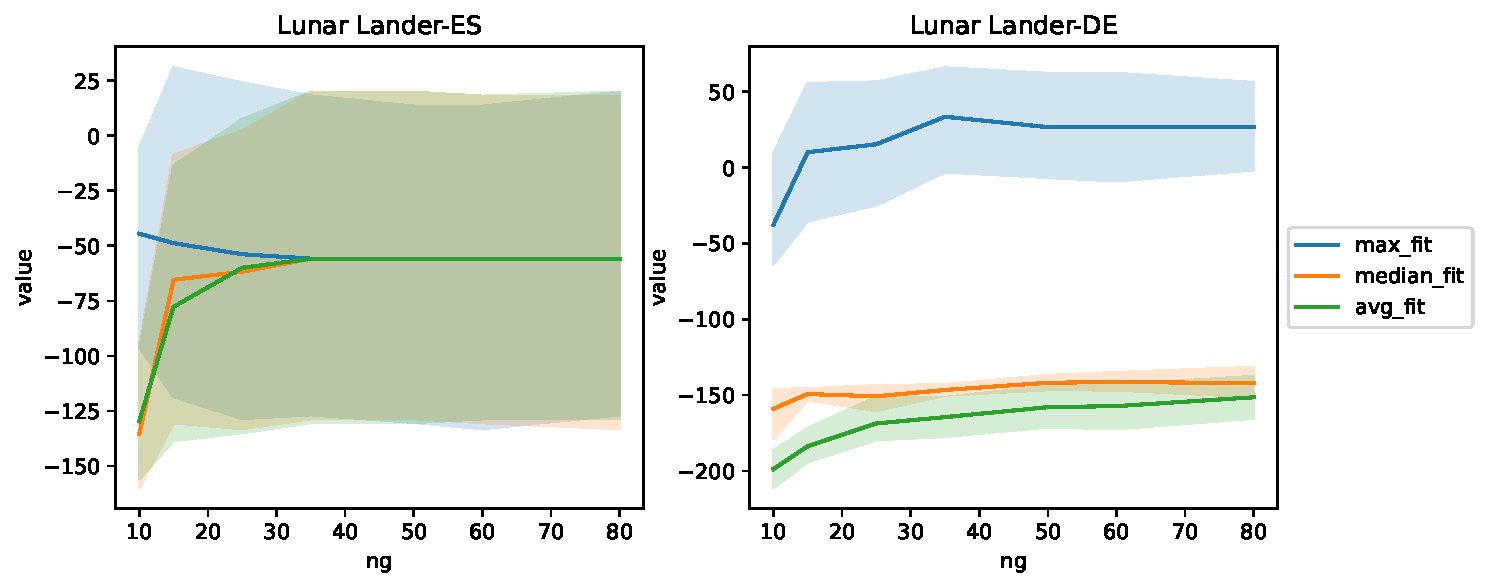
\includegraphics[width=0.9\textwidth]{../img/Origin_generations_lunarlander_fitness}
            \caption{Detailed fitness/generation characteristic for fitness on Lunar Lander env. }
            \label{fig:og_gen_lunarlander_fitness}
            \end{figure}

        
            \begin{figure}[H]
            \centering
            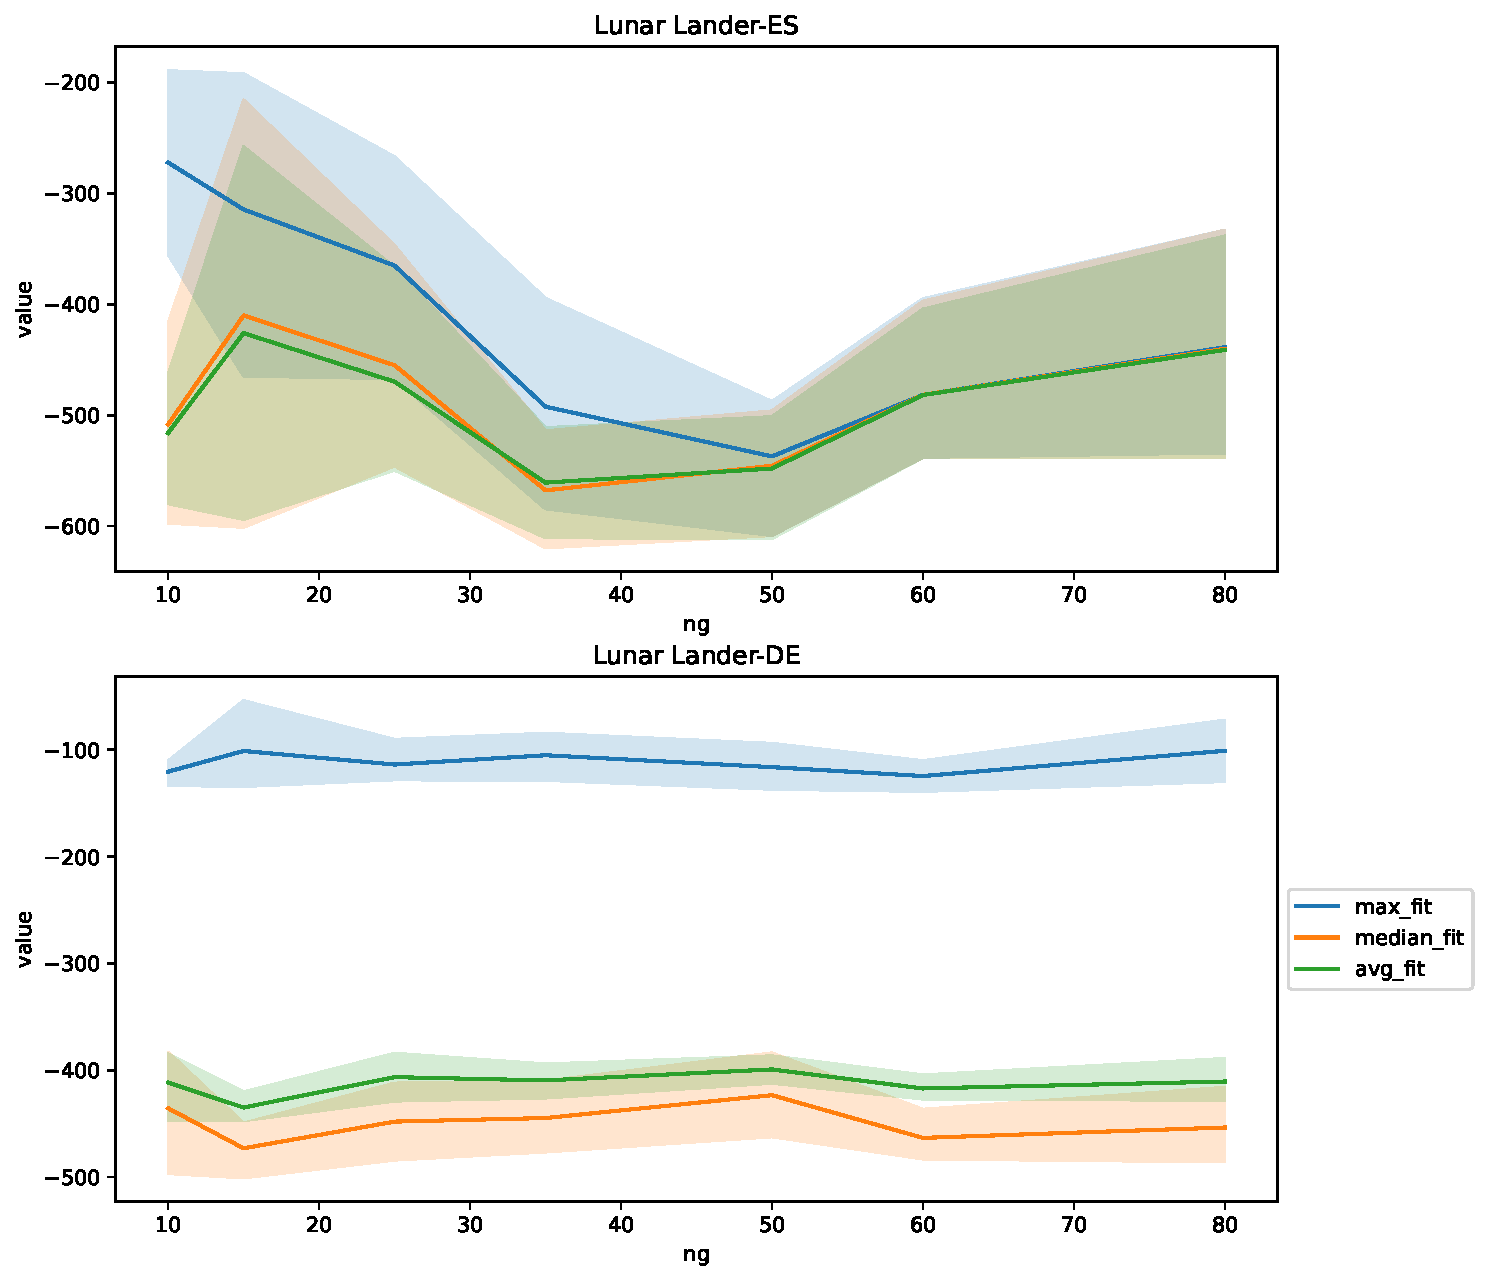
\includegraphics[width=0.9\textwidth]{../img/Origin_generations_lunarlander_novelty}
            \caption{Detailed fitness/generation characteristic for pure novelty on Lunar Lander env. }
            \label{fig:og_gen_lunarlander_novelty}
            \end{figure}

        
            \begin{figure}[H]
            \centering
            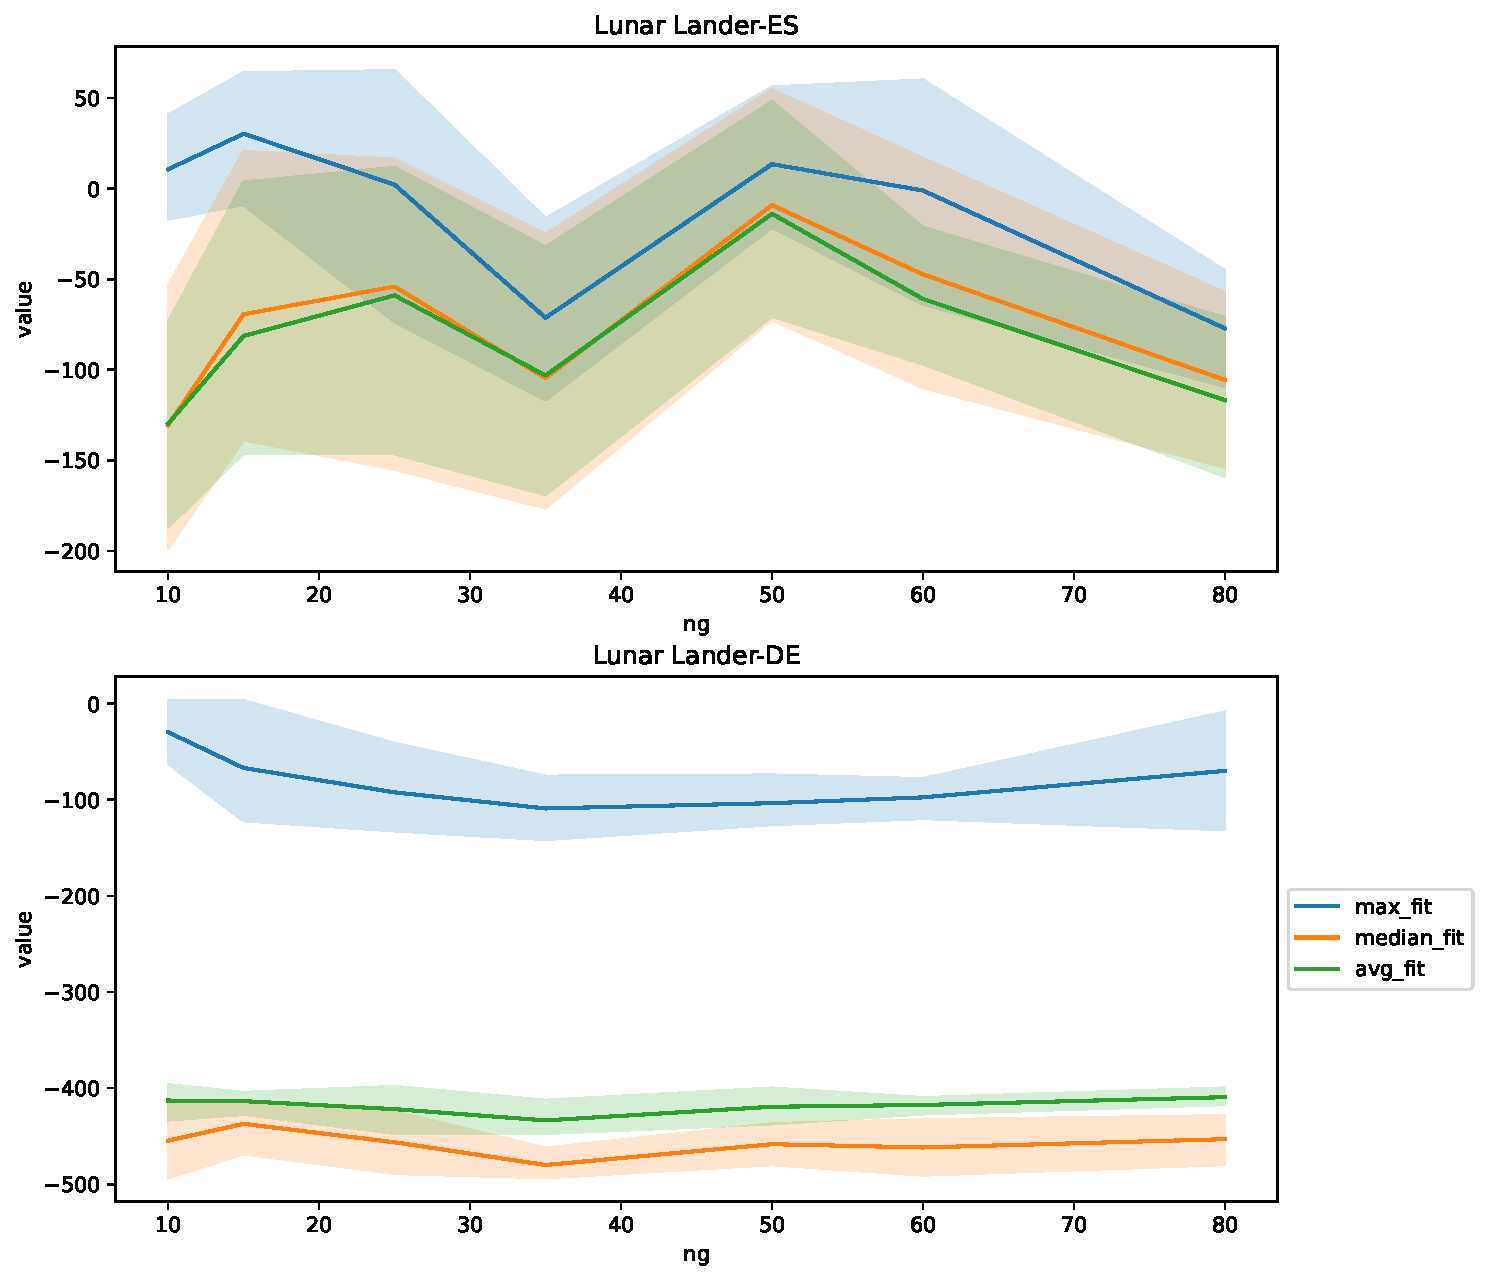
\includegraphics[width=0.9\textwidth]{../img/Origin_generations_lunarlander_add_novelty}
            \caption{Detailed fitness/generation characteristic for inc. fitness on Lunar Lander env. }
            \label{fig:og_gen_lunarlander_add_novelty}
            \end{figure}

        
            \begin{figure}[H]
            \centering
            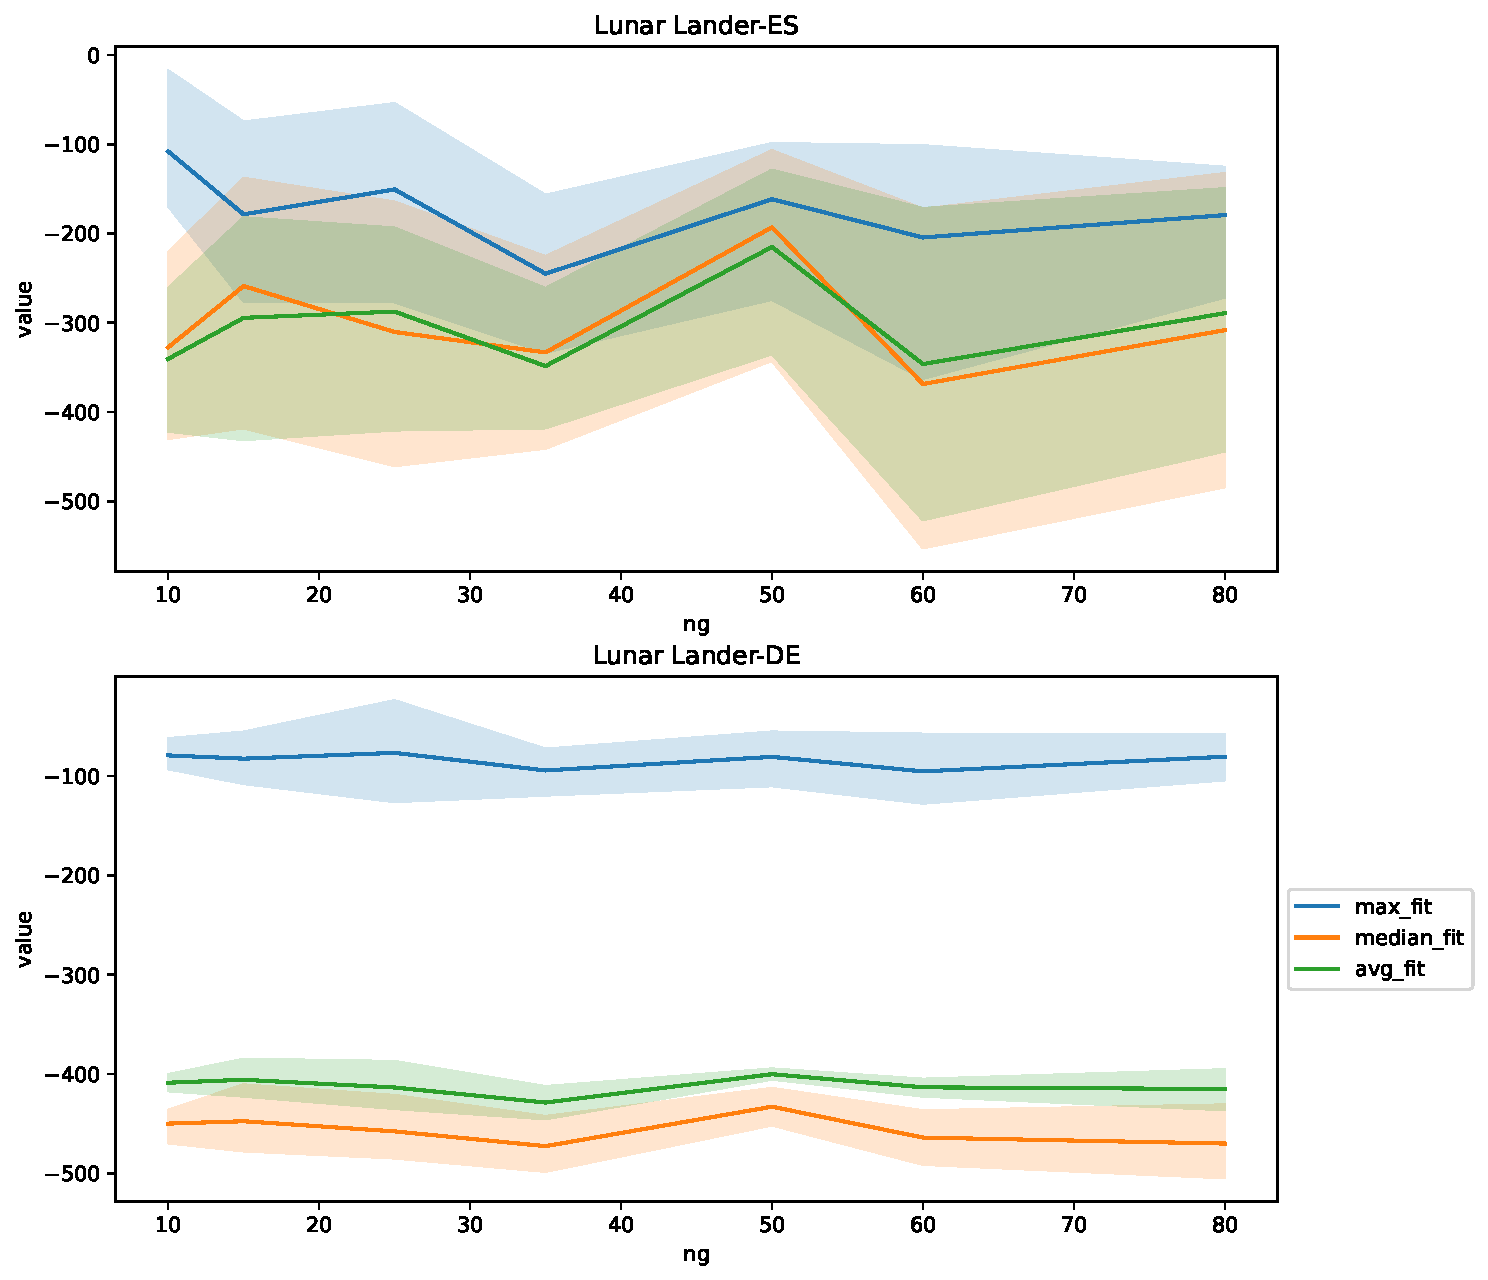
\includegraphics[width=0.9\textwidth]{../img/Origin_generations_lunarlander_sub_novelty}
            \caption{Detailed fitness/generation characteristic for inc. novelty on Lunar Lander env. }
            \label{fig:og_gen_lunarlander_sub_novelty}
            \end{figure}

        
            \begin{figure}[H]
            \centering
            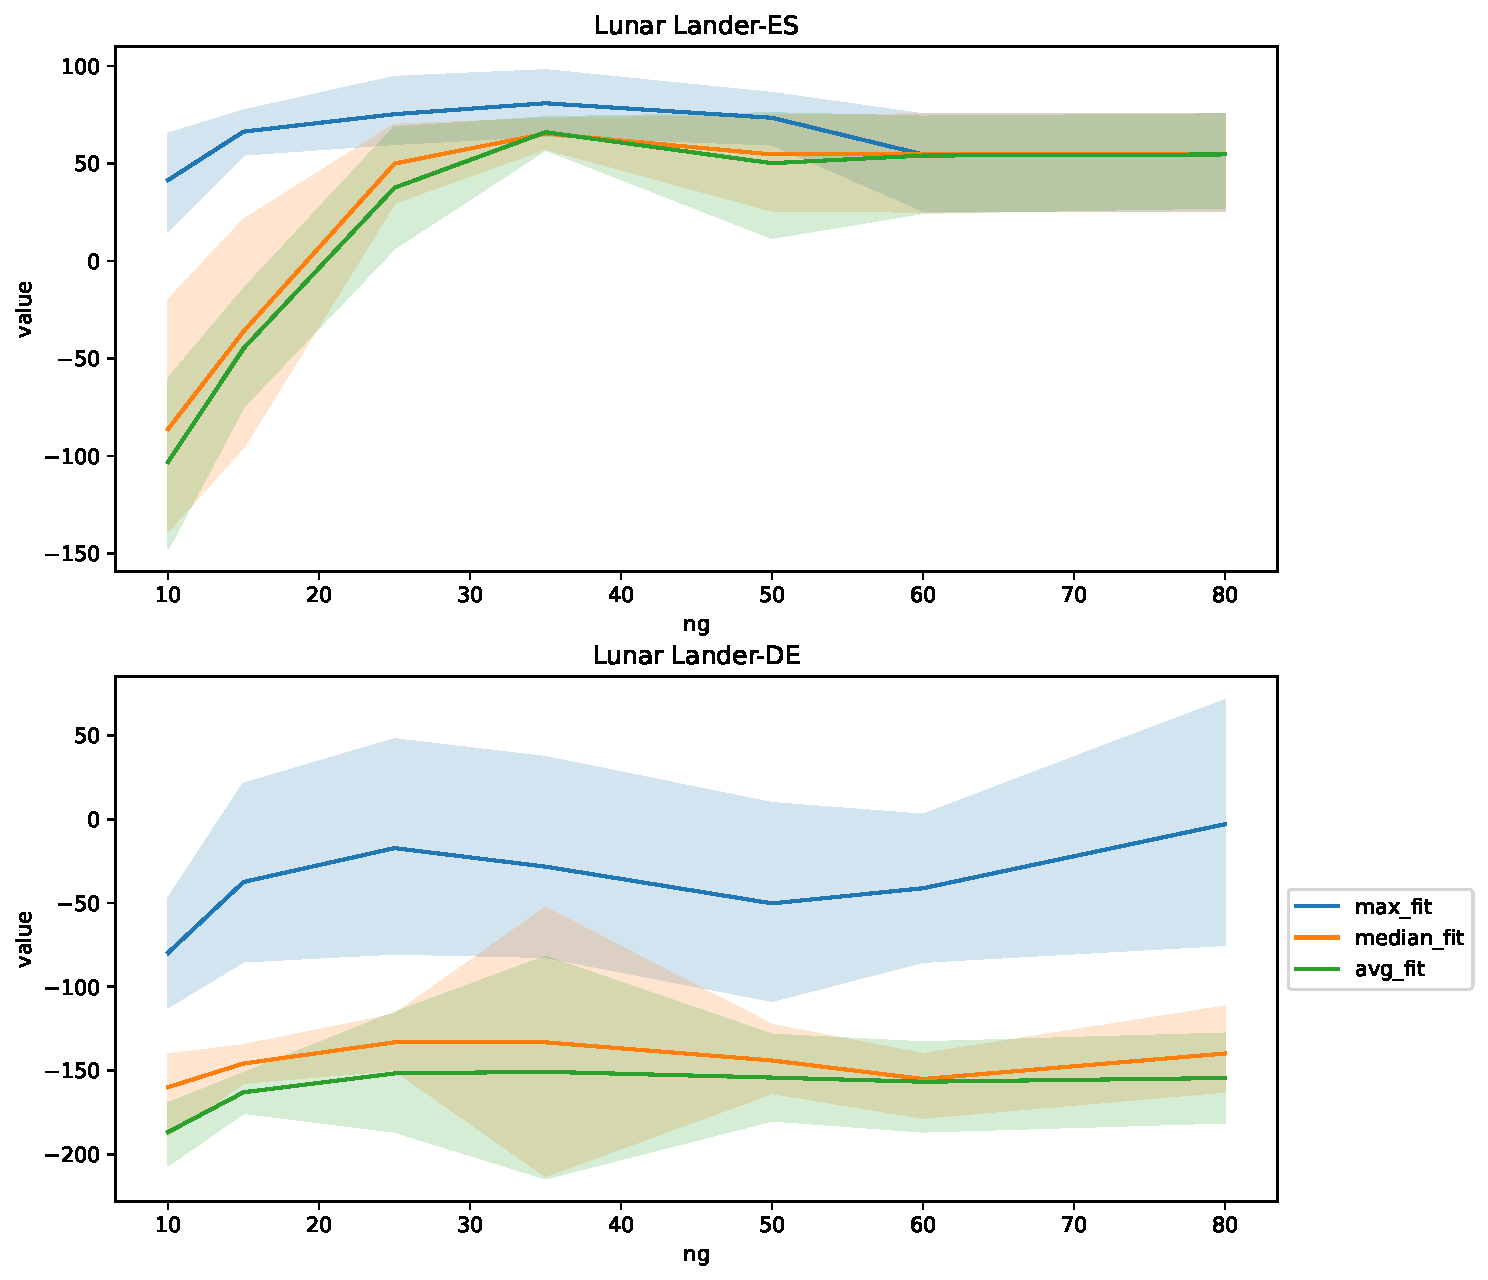
\includegraphics[width=0.9\textwidth]{../img/Origin_generations_lunarlander_fit_archiving}
            \caption{Detailed fitness/generation characteristic for fit. archive on Lunar Lander env. }
            \label{fig:og_gen_lunarlander_fit_archiving}
            \end{figure}

        
            \begin{figure}[H]
            \centering
            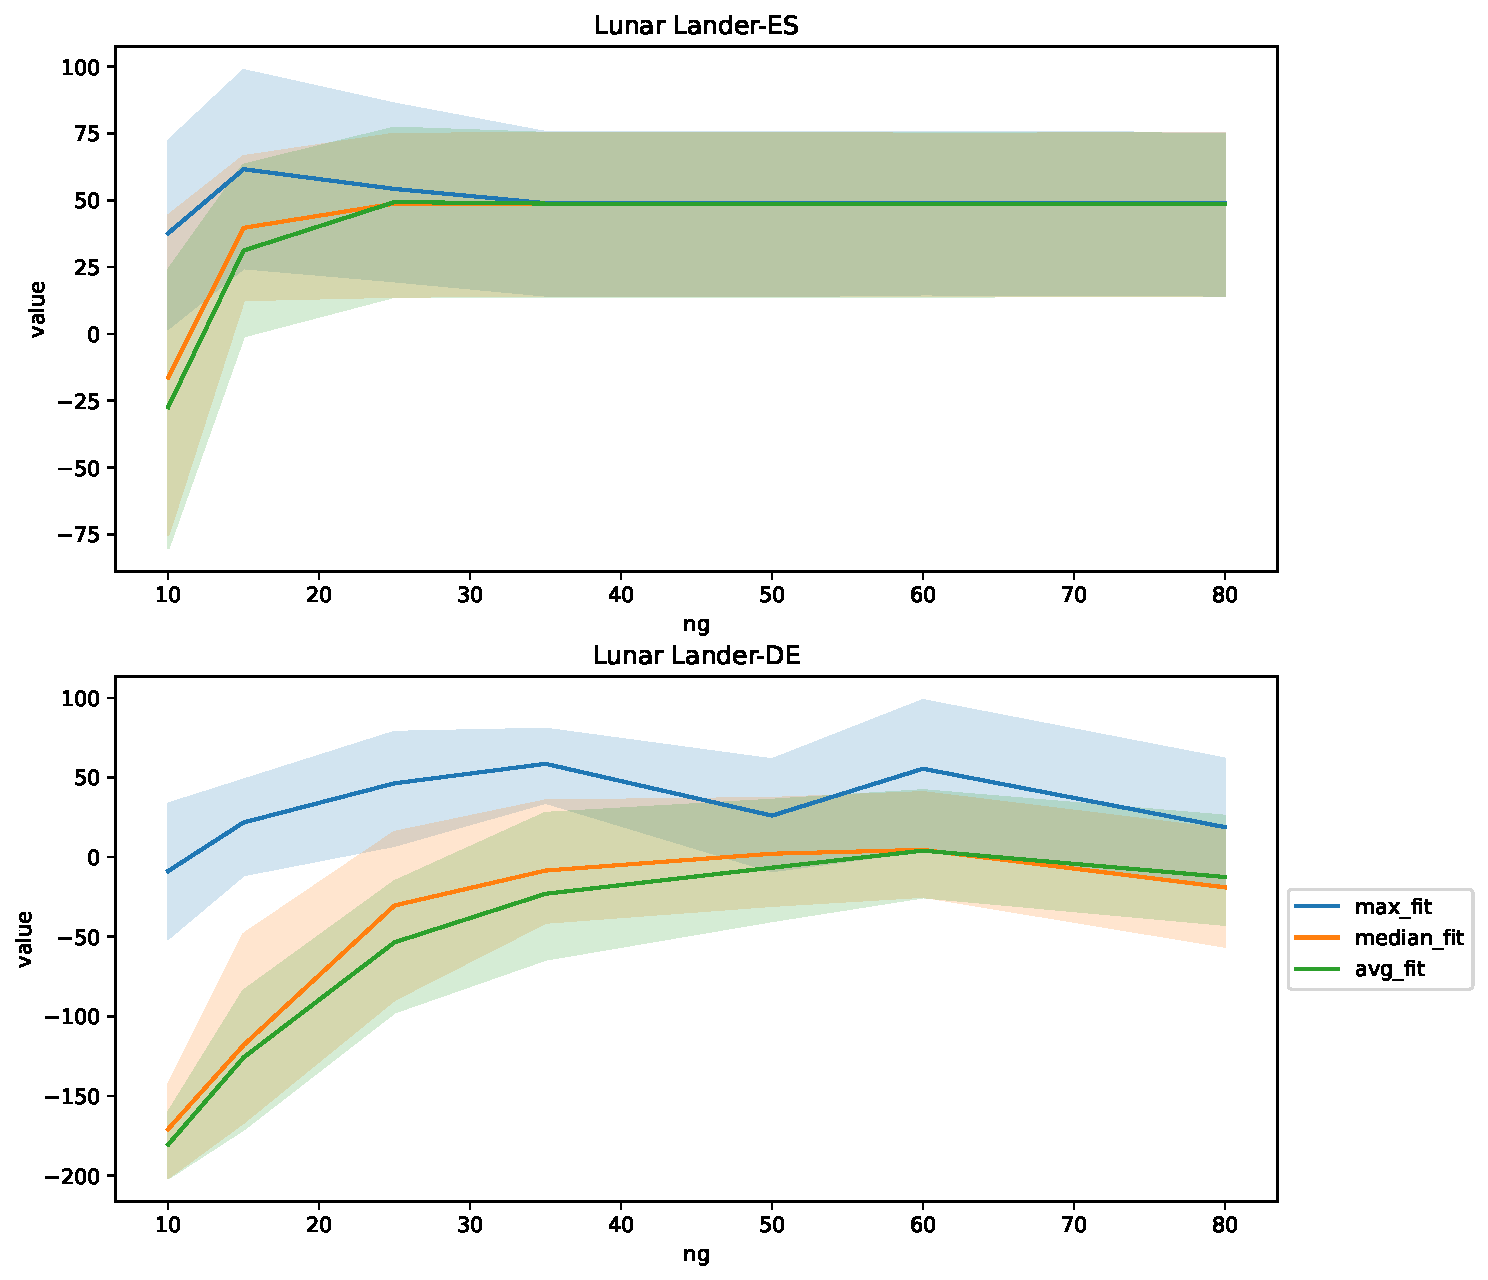
\includegraphics[width=0.9\textwidth]{../img/Origin_generations_lunarlander_elite_archiving}
            \caption{Detailed fitness/generation characteristic for elite archive on Lunar Lander env. }
            \label{fig:og_gen_lunarlander_elite_archiving}
            \end{figure}

        
            \begin{figure}[H]
            \centering
            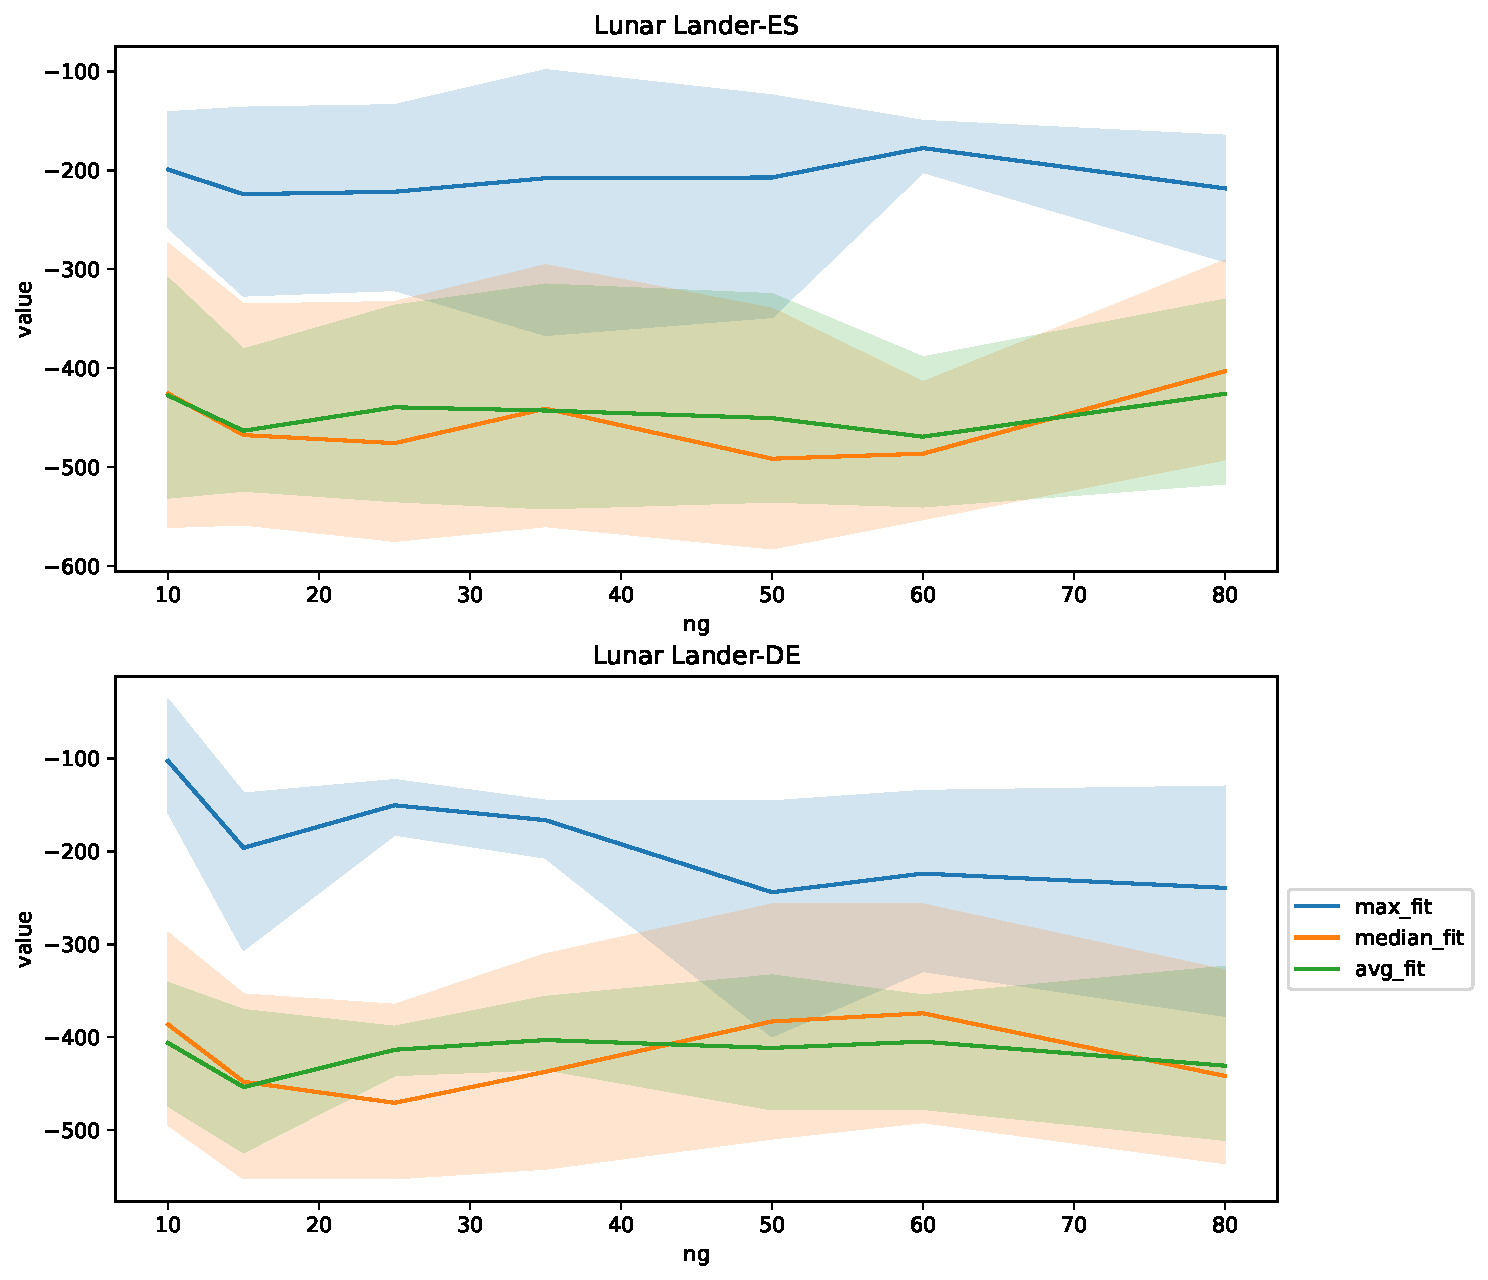
\includegraphics[width=0.9\textwidth]{../img/Origin_generations_lunarlander_novelty_archiving}
            \caption{Detailed fitness/generation characteristic for novelty archive on Lunar Lander env. }
            \label{fig:og_gen_lunarlander_novelty_archiving}
            \end{figure}

        
            \begin{figure}[H]
            \centering
            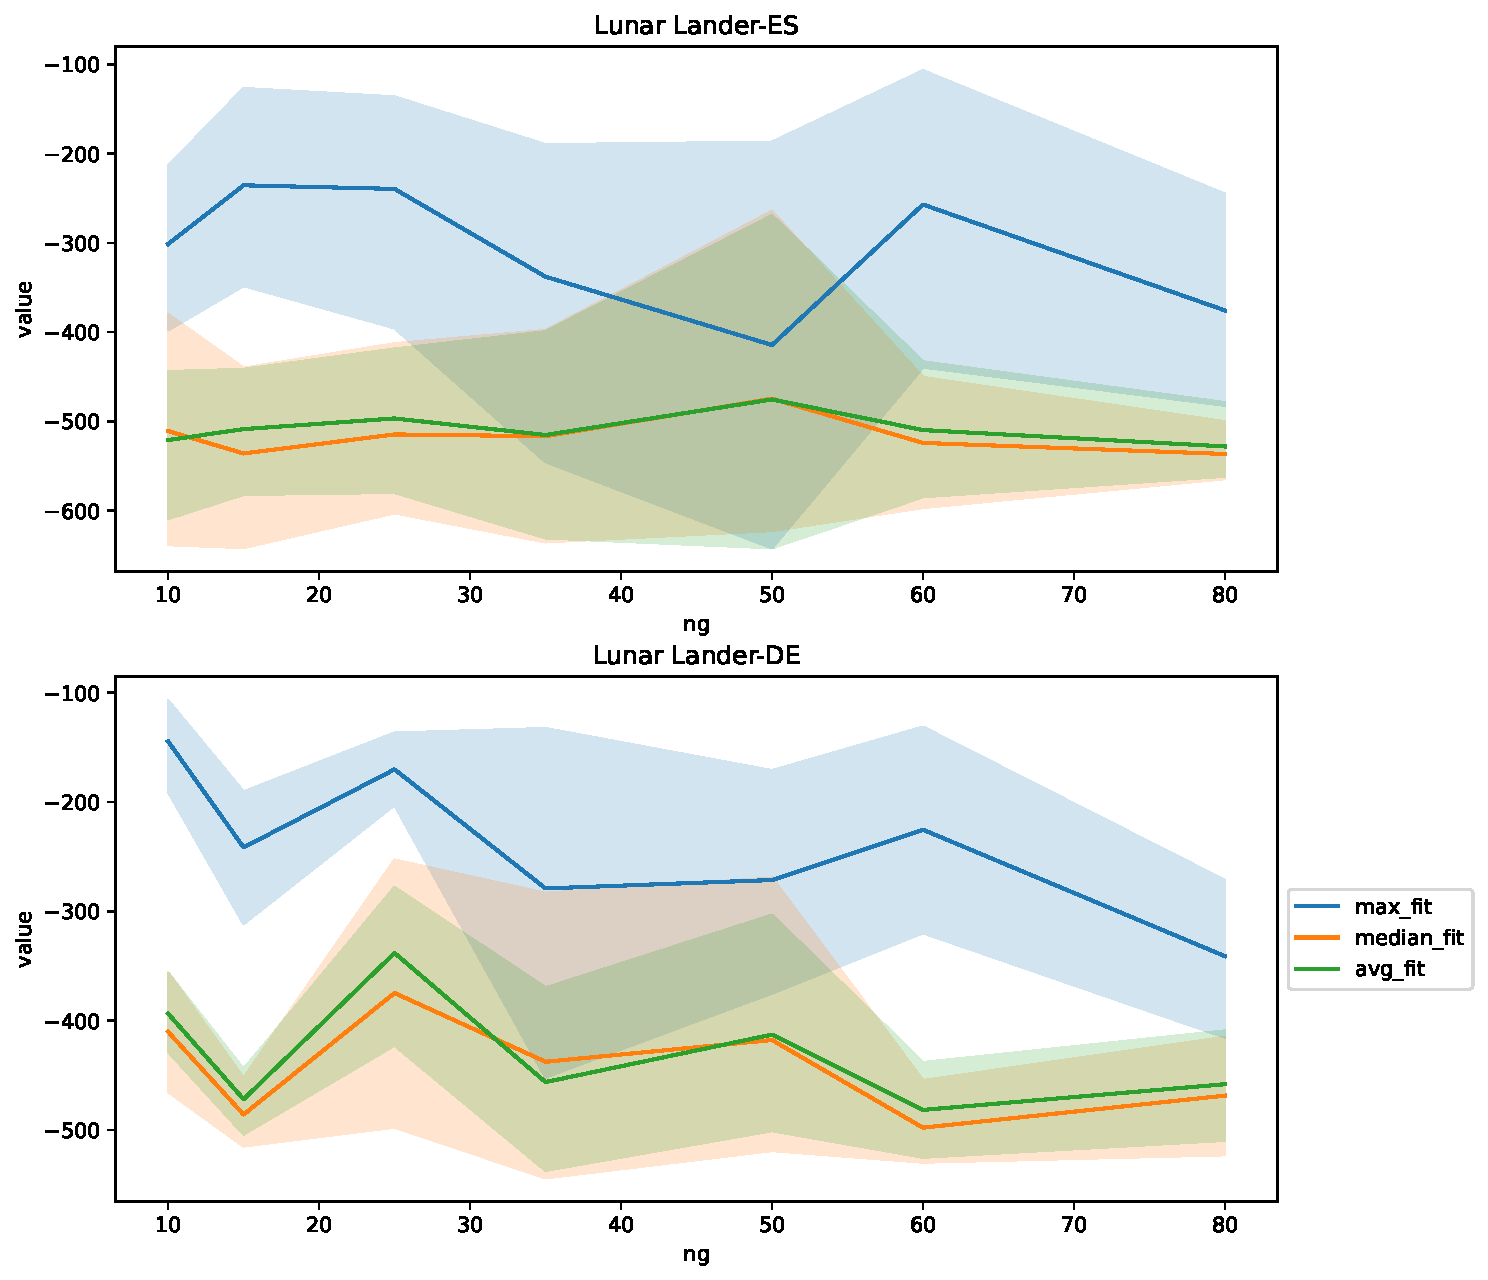
\includegraphics[width=0.9\textwidth]{../img/Origin_generations_lunarlander_novelty_limit}
            \caption{Detailed fitness/generation characteristic for limit archive on Lunar Lander env. }
            \label{fig:og_gen_lunarlander_novelty_limit}
            \end{figure}

        
\section{Project structure}
\begin{figure}[H]
	\centering
	\begin{forest}
		filesystem
		[Project
		[Archive/ \hfill {\normalfont\footnotesize Archived experiments and outputs (unfeatured)}]
		[Data/ \hfill {\normalfont\footnotesize Datasets and generated data}]
		[Docs/ \hfill {\normalfont\footnotesize Thesis \LaTeX{} files}]
		[libs/ \hfill {\normalfont\footnotesize Implementations of the algorithms}]
		[notebooks/ \hfill {\normalfont\footnotesize Helper Jupyter notebooks}]
		[scripts/ \hfill {\normalfont\footnotesize Automation Bash scripts}]
		[adaptive\_gridsearch.py \hfill {\normalfont\footnotesize Incremental grid search}]
		[diff\_cont.py \hfill {\normalfont\footnotesize DE evaluation}]
		[final\_examination.py \hfill {\normalfont\footnotesize Final evaluation}]
		[generation\_examination.py \hfill {\normalfont\footnotesize Generation evaluation}]
		[lambda\_cont.py \hfill {\normalfont\footnotesize ES evaluation}]
		[optuna\_experiment.py \hfill {\normalfont\footnotesize Optuna experiments}]
		[view\_episodes.py \hfill {\normalfont\footnotesize Replay}]
		[visualisation.py \hfill {\normalfont\footnotesize Visualisation utilities}]
		[README.md \hfill {\normalfont\footnotesize Project documentation}]
		]
	\end{forest}
	\caption{Project directory structure.}
	\label{fig:project_structure}
\end{figure}
\section{Experiment Data Format}
\subsection{Incremental Grid Search Protocol}
\begin{lstlisting}[tabsize=3]
	{
		"name": <experiment name>,
		"start": <start timestamp>,
		"end": <end timestamp>,
		
		"origin": [
			<list of hyperparameter sets>
		],
		
		"final": <Final hyperparameter set>,
		
		"visited": [
			<list of hyperparameter sets>	
		]
	}
\end{lstlisting}
\newpage
\subsection{Generations Grid Protocol}

\begin{lstlisting}[tabsize=3]
	{
		"fitness": {
			<# of generations>:{
			
				<seed no.>:[
					[
						[<fitness>], 
						[<behavioral_vector>]
					],
					...,
					[
						[<fitness>], 
						[<behavioral_vector>]
					]
				],
				...
			},
			...
		}
		"environment":<environment id>,
		"algorithm":<algorithm id>,
		"container"<container id>,
		"arguments":{
			<hyperparameter id>: <hyperparameter value>,
			...
		}
	}
\end{lstlisting}
\subsection{Final Experiment Protocol}
\begin{lstlisting}[tabsize=3]
{
	"fitness": {
		<seed no.>:[
			[
				[<fitness>], 
				[<behavioral_vector>]
			],
			...
		],
		...
	}
	"environment":<environment id>,
	"algorithm":<algorithm id>,
	"container"<container id>,
	"arguments":{
		<hyperparameter id>: <hyperparameter value>,
		...
	}
}
\end{lstlisting}
\section{Used Hardware}
\label{app:computers}

\begin{tabular}{ll}
	Lenovo ThinkPad E16 Gen 3 \\
	Lenovo Legion 5\\
	HP ProLiant DL320e Gen8 v2 \\
	
\end{tabular}


\openright
\end{document}
